\documentclass[useAMS,usenatbib]{mn2e}
\usepackage{epsfig,rotate,graphicx}
\usepackage[fleqn]{amsmath}
\usepackage{subfigure}
\usepackage{lscape}
\usepackage{bm}

\newcommand{\p}{\partial}
\newcommand{\mnras}{MNRAS}
\newcommand{\apj}{ApJ}
\newcommand{\aj}{AJ}
\newcommand{\aap}{A\&A}
\newcommand{\apss}{ApSS}
\newcommand{\apjl}{ApJL}
\newcommand{\pasj}{PASJ}
\newcommand{\araa}{ARAA}
\newcommand{\dd}{\delta}
\newcommand{\adot}{\dot{a}}
\newcommand{\be}{\begin{equation}}
\newcommand{\ee}{\end{equation}}
\newcommand{\gtrsim}{\;\raisebox{-.8ex}{$\buildrel{\textstyle>}\over\sim$}\;}
\newcommand{\lesssim}{\; \raisebox{-.8ex}{$\buildrel{\textstyle<}\over\sim$}\;}
\newcommand{\anrev}{{\it ARA\&A, }}
\newcommand{\apjs}{{\it ApJS, }}
\newcommand{\icar}{{\it Icarus, }}
\newcommand{\mnr}{{\it MNRAS, }}
\newcommand{\nat}{{\it Nature, }}
\newcommand{\sci}{{\it Sci, }}
\newcommand{\ana}{{\it A\&A, }}
\newcommand{\anas}{{\it A\&AS, }}
\newcommand{\aaps}{{\it A\&AS, }}
\newcommand{\anar}{{\it A\&AR, }}
\newcommand{\prd}{{\it Phys. Rev. D }}
\newcommand{\qjl}{{\it QJRAS, }}
\newcommand{\sbar}{\bar{\sigma}}
\newcommand{\avg}[1]{\langle #1 \rangle}
\newcommand{\bu}{\bm{u}}
\newcommand{\lmax}{l_\mathrm{max}}
\newcommand{\mmax}{m_\mathrm{max}}
\newcommand{\trel}{t_\mathrm{rel}}
\newcommand{\zeus}{{\tt ZEUS-MP }}
\newcommand{\ii}{\mathrm{i}}
\newcommand{\bv}{\bm{v}}
\newcommand{\rin}{r_\mathrm{in}}
\newcommand{\rout}{r_\mathrm{out}}
\newcommand{\ciso}{c_\mathrm{iso}}
\newcommand{\tbeta}{\tilde{\beta}}
\newcommand{\teta}{\tilde{\eta}}
\newcommand{\tcool}{t_\mathrm{cool}}
\newcommand{\jlin}{j_\mathrm{lin}}
\newcommand{\jlintot}{J_\mathrm{lin}}
\newcommand{\tbg}{T_\mathrm{BG}}
\newcommand{\varA}[1]{{\operatorname{#1}}}
\DeclareMathOperator{\erf}{erf}
\DeclareMathOperator{\real}{Re}
\DeclareMathOperator{\imag}{Im}

\usepackage{array,booktabs,tabularx}
\newcolumntype{R}{>{\centering\arraybackslash}X} % right justified tabularx columns


\title[One-arm spirals]{One-arm spirals in 
  locally isothermal, radially structured self-gravitating discs}     

\author[Lin]{Min-Kai Lin$^{1}$
  \thanks{ minkailin@email.arizona.edu} \\ 
  $^1$Department of Astronomy and Steward Observatory, University of
  Arizona, 933 North Cherry Avenue, Tucson, AZ 85721, USA 
}

\begin{document}

\maketitle
\begin{abstract} 
  We present numerical simulations of astrophysical discs with an 
  imposed temperature profile and in which a sub-portion of it is
  self-gravitating. This might represent, for example, mass  
  built-up in a circumstellar or protoplanetary
  disc at the outer edge of a `dead zone', in which there
  is inefficient magneto-hydrodynamic turbulence to enable accretion. 
  We conduct numerical gravito-hydrodynamic experiments in 2D using
  the FARGO code and in 3D with the ZEUS-MP and PLUTO codes. In such
  discs we observe the development of a 
  spiral mode with azimuthal wavenumber $m=1$ with co-rotation radius 
  outside the bulk of the spiral arm, resulting in a nearly stationary 
  one-arm spiral pattern in the self-gravitating region of the
  disc. The development of this one-arm 
  spiral does not require the movement of  
  the central star, as found in previous studies. Instead, we find it 
  to be associated with the imposed 
  temperature gradient and the radial disc structure. 
  We apply results from existing linear theory and attribute the
  growth of this spiral to the non-conservation of angular momentum
  for non-axisymmetric linear perturbations in discs with a forced temperature
  gradient. This may lead to an unstable exchange of angular momentum between the spiral 
  and the background disc. However, because the interaction does
  not explicitly depend on self-gravity, we speculate it may also
  affect low-frequency one-arm spirals in non-self-gravitating
  discs. 
\end{abstract}

\begin{keywords}
  accretion, accretion discs, hydrodynamics, instabilities, methods: numerical, protoplanetary discs 
\end{keywords}

\section{Introduction}\label{intro}
% Protoplanetary discs are expected to contain complex structures
% \citep{armitage11}, which directly impact planet formation theories.  
An exciting development in the study of circumstellar 
discs is the direct observation of large-scale, non-axisymmmetric
structures within them. These
include lopsided dust distributions 
\citep{marel13,fukagawa13,casassus13,isella13,perez14,follette14} and
spiral arms 
\citep{muto12,grady13,christiaens14,avenhaus14,boccaletti14}. 

% planet is popular answer for spiral structure
The attractive explanation for asymmetries in circumstellar discs is to
invoke disc-planet interaction. In particular, spiral structures
naturally arise from the gravitational interaction between a
planet and the gaseous protoplanetary disc it is embedded in
\citep[see, e.g.][for a recent review]{baruteau13b}. Thus, the
presence of spiral arms in circumstellar discs could be signposts of 
planet formation.  

% but also natural in GI.
However, spiral arms are also naturally associated with global gravitational 
instability (GI) of differentially rotating discs
\citep{goldreich65,laughlin96b,laughlin98,nelson98,lodato05,forgan11}. Large-scale
spiral arms may provide significant angular momentum transport to enable
accretion \citep{lynden-bell72, papaloizou91,balbus99,lodato04}, and
spiral structures due to GI are potentially observable with the Atacama Large 
Millimeter/sub-millimeter Array \citep{cossins10,dipierror14}.   

% when/where does it happen? formation stage/dead zones (special for ppd)
GI can be expected in the earliest stages of 
circumstellar disc formation \citep{kratter10b,inutsuka10,tsukamoto13}. %also
% outer parts  
In the case of protoplanetary discs, which have complex structure
\citep{armitage10}, GI may also occur in `dead
zones' --- sub-portions of the disc where the magneto-rotational
instability is ineffective for angular momentum transport
\citep{gammie96,turner08,landry13} and therefore has reduced mass
accretion. Dead zones may become
self-gravitating with sufficient mass built-up
\citep{armitage01,martin12,martin12b,zhu09,zhu10,zhu10b,bae13,bae14}.   

% original motivation for this work (DZGI) 
Given the wide range of GIs that may occur in  gaseous 
astrophysical discs \citep{papaloizou89,christo92,christo93,hadley11,hadley14}, it would of
theoretical interest to clarify what type of GI is relevant to 
partially self-gravitating discs such as a protoplanetary disc containing a 
massive dead zone. This was indeed the original goal of this project. 
However, our seemingly simple initial disc models
consistently produced \emph{one-armed} spiral structures, despite not 
satisfying the usual requirements to generate them 
(see below). We therefore dedicate this study to verify their origin.     

%brief history of m=1 
%stellar wobble from indiana group 
Single-arm spirals, or eccentric modes, corresponding to perturbations 
with azimuthal wavenumber $m=1$, have received interest in
the context of protoplanetary discs because of their global nature
\citep{adams89,heemskerk92,laughlin96,tremaine01,papaloizou02,hopkins10}. Their development is 
often associated with the unique property of $m=1$ perturbations to
move the central star \citep{shu90}, which may have observable
consequeces \citep{michael10}. 
%these are self-gravitating instabilities

The aforementioned analytical studies have mostly adopted barotropic, smooth disc models. 
In this work, we identify a mechanism to generate one-arm
spiral patterns that is related to a non-barotropic equation of
state and disc structure. Specifically, we find that if the disc temperature or
sound-speed is forced to be a prescribed function of position, then 
one-arm spiral modes grows inside a cavity that results from the
adopted disc structure. 

Our study is based on direct hydrodynamic simulations using three
different grid-based codes, both in two-dimensions (2D) and
three-dimensions (3D). We also apply results from previous linear
theory to explain their growth. We find that, when the disc
temperature is prescribed, the usual statement for the conservation of
angular momentum for linear perturbations acquires a source term
proportional to the temperature gradient which may act to destabilise
$m=1$ perturbations. Although we work with self-gravitating discs, the
source term itself does not depend explicitly on disc self-gravity. Thus, the
destabilisation effect we describe may also operate in
non-self-gravitating discs. 

This paper is organised as follows. In \S\ref{model} we list the
governing equations and describe the disc equilibria under
consideration. \S\ref{methods} describes the hydrodynamic codes
employed in this work and several diagnostic measures. We briefly
review basic results from linear theory in \S\ref{wkb} to aid our
interpretation of numerical simulations.  Our main results are presented in 
\S\ref{results2d} for 2D simulations and \S\ref{results3d} for 3D
simulations, and we further analyse them in \S\ref{discussions}. 
We summarise in \S\ref{summary}, including a discussion on
spectulations for future work. 

\section{Governing equations}\label{model} 
We consider an inviscid fluid disc of mass $M_d$ 
orbiting a central star of mass $M_*$. We will mainly examine 2D
(or razor-thin) discs in favour of numerical 
resolution, but have also carried out some 3D disc
simulations. Hence, for generality we describe the system in
3D, using both cylindrical $(R,\phi,z)$ and spherical polar
coordinates $(r,\theta,\phi)$ centred on the star. 
The governing fluid equations in 3D are  
\begin{align}
  &\frac{\p\rho}{\p t} + \nabla\cdot\left(\rho\bm{v}\right) =
  0,\label{cont_eq}\\
  &\frac{\p\bm{v}}{\p t} + \bm{v}\cdot\nabla\bv = -\frac{1}{\rho}\nabla
  p -\nabla \Phi_\mathrm{tot}\label{mom_eq},\\ 
  & \nabla^2\Phi_d = 4 \pi G \rho \label{poisson}, 
\end{align}
where $\rho$ is the mass density, $\bm{v}$ is the 
fluid velocity (the angular velocity being $\Omega \equiv v_\phi/R$), 
$p$ is the pressure and the total potential
$\Phi_\mathrm{tot} = \Phi_* + \Phi_d$ consists of that from the
central star, 
\begin{align}
  \Phi_*(r) = -\frac{GM_*}{r}, 
\end{align}
where $G$ is the gravitational constant,  and the disc potential
$\Phi_d$. We impose a locally isothermal equation of state 
\begin{align}
  p = c_s^2(R)\rho,
\end{align}
where the sound-speed $c_s$ is given by 
\begin{align}\label{sound-speed}
  % c_s(R) = hR_0\Omega_k(R_0)\left(\frac{R}{R_0}\right)^{-q/2}, 
  c_s(R) = c_{s0}\left(\frac{R}{R_0}\right)^{-q/2}
\end{align}
where $c_{s0} = h R_0\Omega_k(R_0)$ and 
$h$ is the disc aspect-ratio at the reference radius $R=R_0$, 
$\Omega_k=\sqrt{GM_*/R^3}$ is the midplane Keplerian frequency, and
$q$ is the imposed temperature gradient (since, for an ideal gas the
temperature is proportional to $c_s^2$). The vertical disc scale-height is
defined by $H=c_s/\Omega_k$. Thus, a strictly isothermal disc with
$q=0$ has $H\propto R^{3/2}$, and $q=1$ corresponds to a 
 disc with constant $H/R$. 



The 2D disc equations are obtained by replacing $\rho$ with the surface
mass density $\Sigma$, $p$ becomes the vertically-integrated pressure, 
and the 2D fluid velocity $\bm{v}$ is evaluated at the midplane, as are
the forces in the momentum equations. In the Poisson equation, $\rho$ is
replaced by $\Sigma\delta(z)$, where $\delta(z)$ is the
delta function. 



\section{Linear density waves}\label{wkb}

{\bf We describe a key feature of locally isothermal discs that
  enables angular momentum exchange between small disturbances and the
  background disc through an imposed radial temperature gradient. This
  conclusion results from the consideration of angular momentum
  conservation within the framework of linear perturbation theory. 
  For simplicity, in this section we consider 2D discs. 
}

In a linear analysis, one assumes a steady axisymmetric background state, 
which is then perturbed such that
\begin{align}  
  \Sigma \to \Sigma(R) + \delta\Sigma_m(R)\exp{\left[\ii\left(-\sigma t +
        m\phi\right)\right]}, 
\end{align}
and similarly for other variables, where $\sigma=\omega+\ii\gamma$ is
a complex frequency with $\omega$ being the real frequency, 
$\gamma$ the growth rate, and $m$ is an integer. We take $m>0$ without
loss of generality.  


The linearised mass and momentum equations are
\begin{align}
  &-\ii\sbar \delta\Sigma_m = -\frac{1}{R}\frac{d}{dR}\left(R\Sigma\delta
    v_{Rm}\right) - \frac{\ii m \Sigma}{R}\delta v_{\phi m}, \\
  &-\ii\sbar\delta v_{Rm} - 2\Omega \delta v_{\phi m} = -
  c_s^2(R)\frac{d}{dR}\left(\frac{\delta\Sigma_m}{\Sigma}\right) - \frac{d}{dR}\delta\Phi_m,\label{radmom}\\
  & -\ii\sbar\delta v_{\phi m} + \frac{\kappa^2}{2\Omega}\delta v_{Rm} =
  -\frac{\ii m }{R}\left(c_s^2\frac{\delta\Sigma_m}{\Sigma} + \delta\Phi_m\right),
\end{align}
where $\sbar = \sigma - m\Omega$ and $\kappa^2 =
R^{-3}\p_R(R^4\Omega^2)$ is the square of the epicyclic frequency. A
locally isothermal equation of state has been assumed in
Eq. \ref{radmom}.  The linearised Poisson equation is 
\begin{align}
  \nabla^2\delta\Phi_m = 4\pi G \delta\Sigma_m \delta(z). 
\end{align}

These linearised equations can be combined into a single
integro-differential equation eigenvalue problem. We defer a full
{\bf numerical} exploration of the linear problem to a future study. Here, we {\bf
  discuss} some
general properties of the linear perturbations. 

\subsection{Global angular momentum conservation for linear
  perturbations} \label{global_cons}
It can be shown that linear perturbations with $\phi$-dependence in the form
$\exp{(\ii m\phi)}$ satisfies angular momentum conservation
in the form 
\begin{align}\label{angcons}
  \frac{\p \jlin}{\p t} + \nabla\cdot\bm{F} = \tbg, 
\end{align}
\citep[e.g.][]{narayan87,ryu92,lin93b} where
\begin{align}\label{lin_ang_mom_cons}
  \jlin \equiv
  -\frac{m\Sigma}{2}\imag\left(\bm{\xi}^*\cdot\frac{\p\bm{\xi}}{\p
      t} + \Omega \hat{\bm{k}}\cdot\bm{\xi}\times\bm{\xi}^* + \ii
    m \Omega |\bm{\xi}|^2\right) 
\end{align}
is the angular momentum density of the linear disturbance (which may
be positive or negative), $\bm{\xi}$ is the Lagrangian
displacement and $^*$ denotes complex conjugation, and $\bm{F}$ is the
vertically-integrated angular momentum flux consisting of a Reynolds
stress and a gravitational stress \citep{lin11b}. Explicit expressions
for $\bm{\xi}$ can be found in, e.g. \cite{papaloizou85}. 

In Eq. \ref{angcons}, the background torque density $\tbg$ is 
\begin{align}\label{baroclinic_torque}
  \tbg \equiv
  -\frac{m}{2}\imag\left(\delta\Sigma_m\xi_R^*\frac{dc_s^2}{dR}\right), 
\end{align}
and arises because we have adopted a locally isothermal equation of
state {\bf in the perturbed disk}. {\bf  We outline the
derivation of $T_\mathrm{BG}$ in Appendix \ref{tbg_deriv}.} 

In a barotropic fluid, such as a strictly isothermal disc,
$\tbg$ vanishes and the total angular momentum associated with
the perturbation is conserved, provided that there is no net angular
momentum flux. However, as noted in \cite{lin11b}, if there is an imposed
temperature gradient, as in the disc models we consider,
then $\tbg\neq 0$ in general, which corresponds to a local torque
exerted by the background disc on the perturbation. 

The important consequence of the background torque is the possibility
of instability if $\tbg\jlin>0$. That is, if $\jlin$ is positive
(negative) and the background torque $\tbg$ is {\bf also} positive (negative),
then the local angular momentum density of the linear disturbance
{\bf will} further increase (decrease) {\bf with time}. This implies the amplitude of the disturbance
may grow by exchanging angular momentum with the background
disc.

{\bf 
  We demonstrate instability for low-frequency modes 
  ($|\omega|\ll m\Omega$) by explicitly showing its 
  angular momentum density 
  $\jlin<0$, and the background torque $T_\mathrm{BG}<0$ for
  appropriate perturbations and radial temperature gradients. 
}

\subsection{Angular momentum density of  non-axisymmetirc low-frequency modes}
From Eq. \ref{lin_ang_mom_cons} and assuming a time-dependence of the
form $\exp{(-\ii \sigma t)}$ with $\real{\sigma} = \omega$,  
the angular momentum density associated with linear waves is
\begin{align}
  \jlin = \frac{m\Sigma}{2}\left[\left(\omega -
      m\Omega\right)|\bm{\xi}|^2 + \ii\Omega\left(\xi_R\xi_\phi^* -
      \xi_R^*\xi_\phi\right)\right].\label{ang_mom_def}  
\end{align}
For a low-frequency mode, $|\omega|\ll m\Omega$. Then neglecting the
term $\omega|\bm{\xi}|^2$, {\bf we find}
\begin{align}
  \jlin &\simeq \frac{m\Sigma\Omega}{2}\left[-m|\bm{\xi}|^2 + \ii\left(\xi_R\xi_\phi^* -
      \xi_R^*\xi_\phi\right)\right]\notag\\
  & = -\frac{m\Sigma\Omega}{2}\left[ (m-1)|\bm{\xi}|^2 +  |\xi_R + \ii\xi_\phi|^2\right].
%  & \leq 0.
\end{align}
{\bf
Thus, non-axisymmetric ($m\geq1$) low-frequency modes generally have 
negative angular momentum. If the mode loses (positive) angular momentum 
to the background, then we can expect instability. We show 
below how this is possible through a forced temperature
gradient via the background torque. It is simplest to calculate
$T_\mathrm{BG}$ in the local approximation, which we review first.  
}

%and setting $m=1$,
%\begin{align}
 % \jlin &\simeq \frac{\Sigma\Omega}{2}\left[-|\bm{\xi}|^2 + \ii\left(\xi_R\xi_\phi^* -
  %    \xi_R^*\xi_\phi\right)\right]\notag\\
%  & = -\frac{\Sigma\Omega}{2}|\xi_R + \ii\xi_\phi|^2\notag\\
 % & \leq 0.
%\end{align}

\subsection{Local results}\label{local_approx}
In the local approximation, perturbations are assumed to vary rapidly
relative to any background gradients. The
dispersion relation for tightly-wound density 
waves of the form $\exp{[\ii(-\sigma t + m \phi + kR)]}$ in a razor-thin
disc is  
\begin{align}\label{dispersion}
  (\sigma - m\Omega)^2 = \kappa^2 + k^2c_s^2 - 2\pi G \Sigma |k|, 
\end{align}
where $k$ is a real wavenumber such that $|kR|\gg1$ \citep{shu91}. 
Note that in the {\bf strictly} local approximation, {\bf where all
  global effects are neglected}, only axisymmetric perturbations
($m=0$) can be unstable. % (having an imaginary $\sigma$).     

Given the real frequency $\omega$ or pattern speed $\Omega_p\equiv  
\omega/m$ of a {\bf non-axisymmetric} neutral mode 
, Eq. \ref{dispersion} can be solved 
for $|k|$, 
\begin{align}\label{wavenumber}
%  |k| = \frac{\pi G \Sigma}{c_s^2}\left[1 \pm \sqrt{1 -
 %     Q^2(1-\nu^2)}\right], 
|k| = k_c\left[1 \pm \sqrt{1 -
     Q^2(1-\nu^2)}\right], 
\end{align}
where 
 \begin{align}
   k_c \equiv \frac{\pi G \Sigma}{c_s^2}
 \end{align}
 is a characteristic wavenumber, 
\begin{align}
  Q \equiv \frac{c_s\kappa}{\pi G \Sigma}
\end{align}
is the usual Toomre parameter, and
\begin{align}
  \nu \equiv \frac{(\omega - m\Omega)}{\kappa}
\end{align}
is a dimensionless frequency. In
Eq. \ref{wavenumber}, the upper (lower) sign correspond to short
(long) waves, and $k>0$ ($k<0$) correspond to trailing (leading)
waves.    

{\bf At the \emph{co-rotation radius} $R_c$} the pattern speed matches
the fluid rotation,
\begin{align}
  \Omega(R_c) = \Omega_p.
\end{align}
\emph{Lindblad resonances} $R_L$ occurs where
\begin{align}
  \nu^2(R_L) = 1. 
\end{align}
Finally, \emph{Q-barriers} occur at radii $R_{Qb}$ where
\begin{align}
  Q^2(R_{Qb})\left[1-\nu^2(R_{Qb})\right] = 1.  
\end{align}
According to Eq. \ref{wavenumber}, purely wave-like solutions with
real $k$ are only possible where $Q^2(1-\nu^2)\leq1$.  

A detailed discussion of the properties of local density waves 
is given in \cite{shu91}. An important result, {\bf which holds for
  waves of all frequencies}, is that
waves interior to co-rotation ($R<R_c$) have negative angular momentum, while
waves outside co-rotation ($R>R_c$) have positive angular
momentum. 

\subsection{Unstable interaction between low-frequency modes 
  and the background disc due to an imposed temperature gradient}
{\bf 
Here we show that the torque density acting on a low-frequency, 
local mode due to the background temperature gradient can be negative, which 
would enforce the mode, because it has negative angular momentum.  
}

The Eulerian surface density perturbation is given by
\begin{align}\label{den_pert}
  \delta\Sigma_m = -\nabla\cdot\left(\Sigma\bm{\xi}\right) 
  = -\frac{1}{R}\frac{d}{dR}\left(R\Sigma \xi_R\right) - \frac{\ii m}{R}\Sigma\xi_\phi.  
\end{align}
We invoke local theory by setting $d/dR \to \ii k$ where $k$ is
real, and assume $|kR|\gg m$ so that the second term on the right hand
side of Eq. \ref{den_pert} can be neglected. Then    
\begin{align}
  \delta\Sigma _m  \simeq -\ii k \Sigma \xi_R.
\end{align}
{\bf Inserting this into the expression for the background torque,
  Eq. \ref{baroclinic_torque}, we find}
\begin{align}
  T_\mathrm{BG} = \frac{m}{2}\frac{dc_s^2}{dR}k\Sigma |\xi_R|^2. \label{baroclinic_torque1}
\end{align}


This torque density is negative for trailing waves ($k>0$) in discs with
a fixed temperature profile decreasing outwards ($dc_s^2/dR<0$). Note
that this conclusion does not rely on the low-frequency approximation.    

However, if the linear disturbance under consideration \emph{is} a
low-frequency mode, then it has negative angular
momentum. If it is trailing and $dc_s^2/dR<0$, as is typical
in astrophysical discs, then $T_\mathrm{BG}<0$, and
the background disc applies a negative torque on the disturbance,
which further decreases its angular momentum. This suggests the {\bf
  mode} 
amplitude will grow.  

Using $\jlin$ and $T_\mathrm{BG}$, we can estimate the 
growth rate $\gamma$ of linear perturbations due to the background
torque as  
\begin{align}
  2\gamma \sim \frac{T_\mathrm{BG}}{\jlin},
\end{align}
where the factor of two accounts for the fact that the angular momentum
density is quadratic in the linear perturbations. Inserting the above
expressions for $\jlin$ and $T_\mathrm{BG}$ for gives
\begin{align}\label{theoretical_rate0}
  2\gamma \sim
  -\frac{dc_s^2}{dR}
  \frac{k}{\Omega}\frac{|\xi_R|^2}{\left[(m-1)|\bm{\xi}|^2 + |\xi_R +
      \ii\xi_\phi|^2 \right]} 
  = -\frac{dc_s^2}{dR}
  \frac{k}{m\Omega},
%  -\frac{dc_s^2}{dR}\frac{k}{\Omega}\frac{|\xi_R|^2}{|\xi_R + \ii
%   \xi_\phi|^2}. 
\end{align}
{\bf where the second equality uses $\xi_\phi \simeq
2\ii \xi_R/m$ in the local approximation, as shown in  Appendix
\ref{horizontal_displacements}.} 
Then for the temperature profiles $c_s^2 = c_{s0}^2 (R/R_0)^{-q}$ as
adopted in our disc models,  
\begin{align}
  2\gamma \sim q\frac{c_s^2}{R}\frac{k}{m\Omega} \sim q h
  \left(\frac{kH}{m}\right)\Omega,\label{theoretical_rate}
\end{align}
where we used $c_s\sim H\Omega\sim hR\Omega$. {\bf
  Eq. \ref{theoretical_rate} suggests that perturbations with small
  radial length-scales ($kH\gtrsim m$) are most favourable for
  destabilisation. Taking the local approximation is then
  appropriate.}       


{\bf Note that the derivation of Eq. \ref{baroclinic_torque1} and 
  Eq. \ref{theoretical_rate} do not 
  require the disc to be self-gravitating. Thus, destabilisation by the
  background torque is not directly associated with disc
  self-gravity. However, in order to evaluate 
  Eq. \ref{baroclinic_torque1} or Eq. \ref{theoretical_rate} in terms 
  of disc parameters (as done in \S\ref{fargo_m1}), we need to insert a 
  value of $k$, which may depend on disc    
  self-gravity (e.g. from Eq. \ref{wavenumber}).  
}   


\section{Numerical simulations}\label{methods}

{\bf
  We demonstrate the destabilising effect of a fixed temperature
  gradient using numerical simulations. The above discussion is
  generic for low-frequency non-axisymmetric modes, but for
  simulations we will consider specific examples.  
  
  There are two components to the destabilising mechanism.  First
  the disc should support low-frequency modes, which is then
  destabilised by an imposed temperature gradient. The latter is
  straight forward to implement by adopting a locally isothermal
  equation of state as described in \S\ref{model}.  For the former, we
  consider discs with a  
  radially-structured Toomre $Q$ profile. We use local theory to show that such discs support
  low-frequency trapped one-armed ($m=1$) modes. 
  This is convenient because Eq. \ref{theoretical_rate} indicates that
  modes with small $m$ are
  more favourable for destabilisation by an imposed temperature
  gradient.  
}


\subsection{Disc model and initial conditions}
For the initial disc profile we adopt a modified power-law disc with
surface density given by
\begin{align}
  \Sigma(R) = \Sigma_\mathrm{ref} \left(\frac{R}{R_0}\right)^{-s}\times B(R;
  R_{1}, R_{2}, \epsilon, \delta R), 
\end{align}
where $s$ is the power-law index describing the smooth disc and
$\Sigma_\mathrm{ref}$ is a 
surface density scale chosen by specifying $Q_\mathrm{out}$,
the Keplerian Toomre parameter at $R=R_{2}$,
\begin{align}
  Q_\mathrm{out} = \left.\frac{c_s\Omega_k}{\pi G
    \Sigma}\right|_{R=R_{2}}. 
\end{align}
The bump function
$B(R)$ represents a surface density boost between
$R\in[R_{1},R_{2}]$ by a factor $\epsilon^{-1}>1$,
and $\delta R$ is the transition width between the bump and the
smooth disc. We choose 
\begin{align}\label{sig_bump}
  &B(R) = f_1(R)\times f_2(R),\\
  &f_1(R) = \frac{1}{2}\left(1 - \epsilon\right)\left[1 +
    \tanh\left(\frac{R-R_{1}}{\Delta_1}\right)\right]  + \epsilon,\\
  &f_2(R) = \frac{1}{2}\left(1 - \epsilon\right)\left[1 -
    \tanh\left(\frac{R-R_{2}}{\Delta_2}\right)\right]  + \epsilon,
\end{align}
where $\Delta_{1,2} = \delta R \times H(R_{1,2})$. 

The 3D disc structure is obtained by assuming vertical hydrostatic
balance  
\begin{align}
  0 = \frac{1}{\rho}\frac{\p p}{\p z} + \frac{\p\Phi_*}{\p z} + \frac{\p
    \Phi_d}{\p z},  
\end{align}
which gives the mass density as 
\begin{align}
  \rho = \frac{\Sigma}{\sqrt{2\pi}H}Z(R,z),
\end{align}
where $Z(R,z)$ describes vertical stratification. In practice, we
numerically solve for $Z(R,z)$ by neglecting the radial self-gravity
force compared to vertical self-gravity, which reduces the equations
for vertical hydrostatic equilibrium to ordinary differential
equations. This procedure is described in \cite{lin12b}. 

Our fiducial parameter values are: $s=2$, $R_{1}=R_0$, $R_{2}=2R_0$,
$\epsilon=0.1$, $\delta R=5$, $h=0.05$ and
$Q_\mathrm{out}=2$. An example of the initial surface density and the
Toomre $Q$ parameter is shown in
Fig. \ref{initial_surf}. Since $Q>1$, the disc is stable to local
axisymmetric perturbations \citep{toomre64}. %min Q is 1.3
The transition between self-gravitating and 
non-self-gravitating portions of the disc occur smoothly across
$\sim10H$. Initially there is no vertical or radial velocity
($v_R = v_r = v_\theta = 0$). The azimuthal velocity is initialized to
satisfy centrifugal balance with pressure and gravity,
\begin{align}
  \frac{v_\phi^2}{r} = \frac{1}{\rho}\frac{\p p}{\p r} + \frac{\p
    \Phi_\mathrm{tot}}{\p r}
\end{align}
and similarly in 2D.  

\begin{figure}
  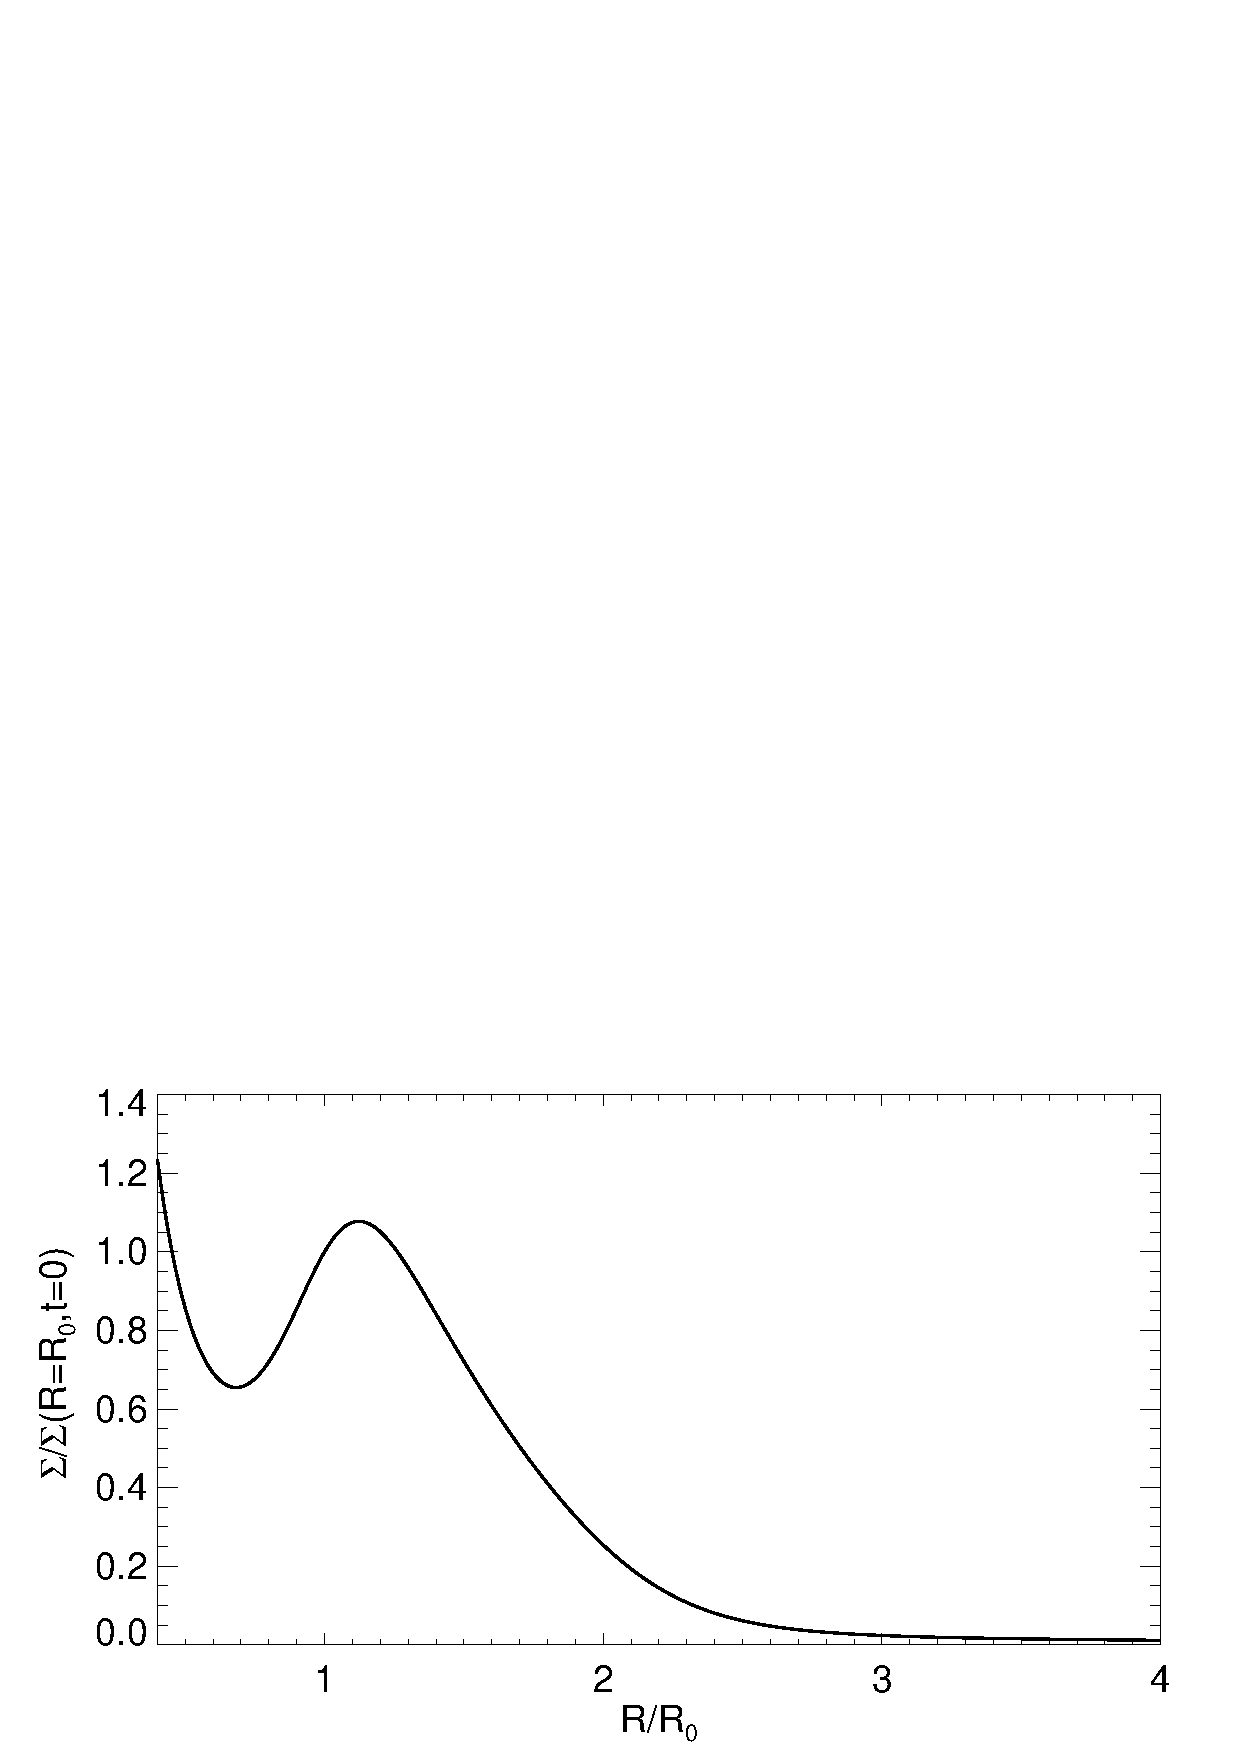
\includegraphics[width=\linewidth,clip=true,trim=0cm 1.7cm 0cm
  0cm]{figures/compare_profiles_dens000} 
  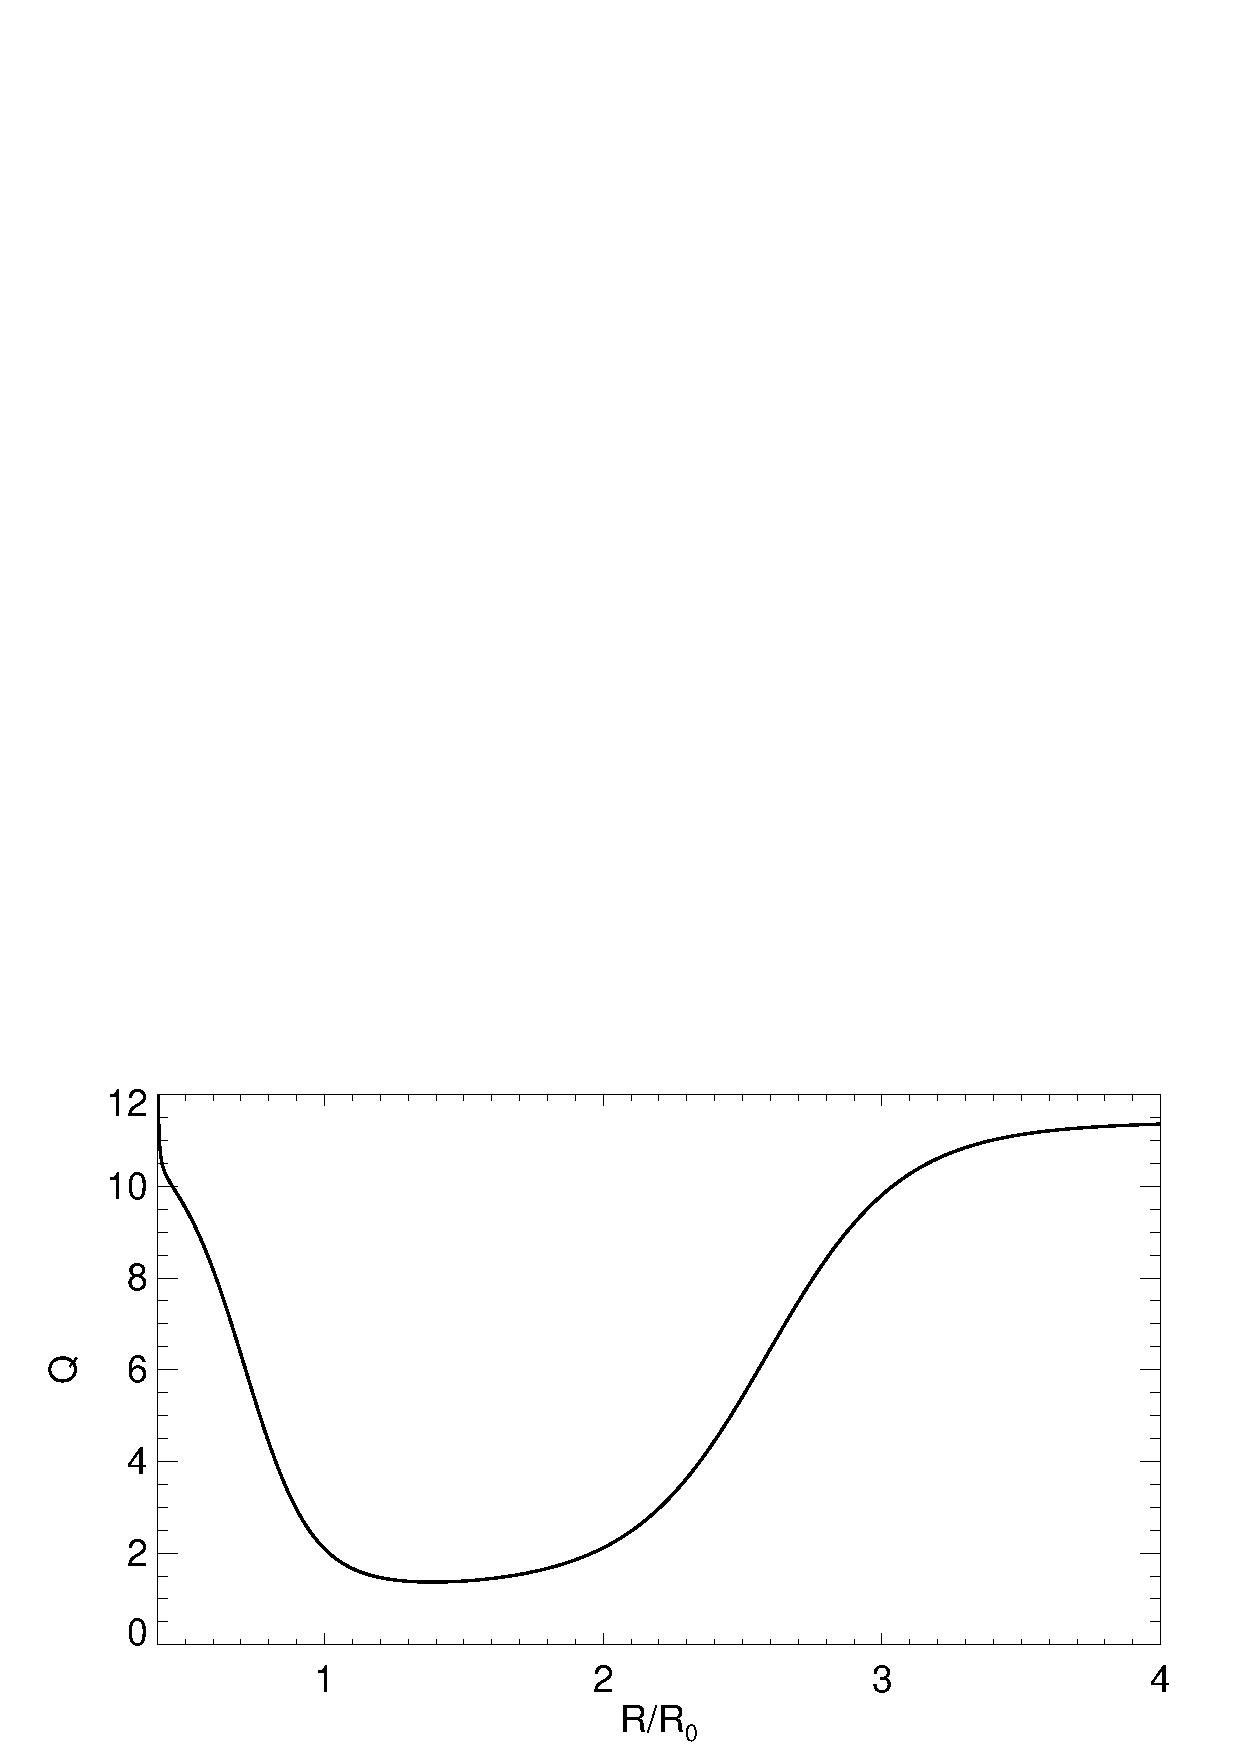
\includegraphics[width=\linewidth]{figures/compare_profiles_Q000}
  \caption{Fiducial profiles of the surface density (top) and Toomre
    parameter (bottom) used in this work.\label{initial_surf}}
\end{figure}

\subsection{Codes}
{\bf We use three independent grid-based codes to simulate the above 
system.} We adopt computational units such that
$G=M_*=R_0=1$. Time is measured  in the Keplerian orbital period at
the reference radius, $P_0\equiv  2\pi/\Omega_k(R_0)$.   

\subsubsection{FARGO}
Our primary code is FARGO with self-gravity \citep{baruteau08}. This
is a popular, simple finite-difference code for 2D discs. `FARGO' refers
to its azimuthal transport algorithm, which removes the mean azimuthal
velocity of the disc, thereby permit larger timesteps than that would otherwise be allowed
by the usual Courant condition based on the full azimuthal
velocity \citep{masset00a,masset00b}.     

The 2D disc occupies
$R\in[R_\mathrm{min},R_\mathrm{max}],\,\phi\in[0,2\pi]$ and is  
divided into $(N_R,N_\phi)$ grids, logarithmically spaced in radius and
uniformly spaced in azimuth. At radial boundaries we set the
hydrodynamic variables to their initial values.   

The 2D Poisson equation is solved in integral form, 
\begin{align}\label{2d_grav}
  &\Phi_{d,z=0}(R,\phi) \notag \\
  &=-\int_{R_\mathrm{min}}^{R_\mathrm{max}} \int_0^{2\pi}
  \frac{G\Sigma(R^\prime,\phi^\prime)R^\prime dR^\prime d\phi^\prime}{\sqrt{R^2+R^{\prime 2} -
      2RR^\prime\cos{(\phi - \phi^\prime)} + \epsilon_g^2}}, 
\end{align}
using Fast Fourier Transform (FFT), where $\epsilon_g$ is a softening
length to prevent a numerical singularity. The FFT approach requires
$\epsilon_g\propto R$ \citep{baruteau08}. In FARGO, $\epsilon_g$ is
set to a fraction of $hR$.  

% poisson kernal integration, softening 
% where used?
% BC
\subsubsection{ZEUS-MP}
ZEUS-MP  is a general-purpose finite difference
code \citep{hayes06}. We use the code in 3D spherical geometry, covering
$r\in[r_\mathrm{min},r_\mathrm{max}]$, $\theta\in[\theta_\mathrm{min},\pi/2]$,
$\phi\in[0,2\pi]$. The vertical domain is chosen to cover $n_H$
scale-heights at $R=R_0$, i.e. $\tan{(\pi/2 - \theta_\mathrm{min})}/h=n_H$. 
The grid is logarithmically spaced in radius and uniformly spaced in the angular
coordinates. We assume symmetry across the midplane, and
apply reflective boundary conditions at radial boundaries and the
upper disc boundary.  

ZEUS-MP solves the 3D Poisson equation using a conjugate gradient
method. To supply boundary conditions to the linear solver, we
expand the boundary potential in spherical harmonics $Y_{lm}$ 
as described in \cite{boss80}. The expansion is truncated at
$(l,m)=(\lmax,\mmax)$. This code was used in \cite{lin12b} for
self-gravitating disc-planet simulations.  

%used in lin 2012 
\subsubsection{PLUTO} 
PLUTO is a general-purpose Godunov code \citep{mignone07}. The grid
setup is the same as that adopted in ZEUS-MP above. We configure the
code similarly to that used in \cite{lin14}: piece-wise linear
reconstruction, a Roe solver and second order Runge-Kutta time
integration. We also enable the FARGO algorithm for azimuthal
transport. 

We solve the 3D Poisson equation throughout the domain using spherical
harmonic expansion \citep{boss80}, as used for the boundary potential
in ZEUS-MP. This version of PLUTO was used in \cite{lin14b} for
self-gravitating disc-planet simulations, producing similar results to
that of ZEUS-MP and FARGO.   

%used in conference proceeding 

\subsection{Diagnostics}

\subsubsection{Evolution of non-axisymmetric modes}
The disc evolution is quantified using mode amplitudes and angular
momenta as follows. We list the 2D definitions with obvious 3D generalisations. 
A hydrodynamic variable $f$ (e.g. $\Sigma$) is written as 
\begin{align}
  f(R,\phi,t) &= \sum_{m=-\infty}^{\infty}f_m(R,t)\exp{\ii m \phi} \notag\\
  &= f_0 + 2 \real\left[\sum_{m=1}^\infty f_m \exp{(\ii
      m\phi)}\right], 
\end{align}
where the $f_m$ may be obtained from Fourier transform in $\phi$. 

The normalised surface density with azimuthal wavenumber $m$ is
\begin{align}
  \Delta\Sigma_m = \frac{2}{\Sigma_{00}} \real\left[\Sigma_m \exp{(\ii
      m\phi)}\right]
\end{align}
where $\Sigma_{00} = \Sigma_0(t=0)$. The time evolution of the
$m^\mathrm{th}$ mode can be characterized by 
assuming $\Sigma_m\propto\exp{(-\ii \sigma t)}$ as in linear
theory. 
%where
%$\sigma = \omega + \ii\gamma$ is a complex frequency, $\omega$ being 
%the real frequency and $\gamma$ is the growth rate. 
The total non-axisymmetric surface density is 
\begin{align}
  \Delta\Sigma = \frac{\Sigma - \Sigma_0}{\Sigma_0}. 
\end{align}

\subsubsection{Angular momentum decomposition}
The total disc angular momentum is
\begin{align}
  J &= \int_{R_\mathrm{min}}^{R_\mathrm{max}}\int_0^{2\pi} \Sigma Rv_\phi RdRd\phi \notag\\
  &= 2\pi\int_{R_\mathrm{min}}^{R_\mathrm{max}} R\Sigma_0 v_{\phi0} R dR \notag\\ 
  &\phantom{=}+
  \sum_{m=1}^\infty2\pi\int_{R_\mathrm{min}}^{R_\mathrm{max}} 2R\real\left[\Sigma_m v_{\phi
      m}^*\right] RdR 
  %&= \sum_{m=0}^\infty \int _{R_\mathrm{min}}^{R_\mathrm{max}}  j_m(R)
  %dR 
  = \sum_{m=0}^\infty J_m. 
\end{align}
We will refer to $J_m$ as the
$m^\mathrm{th}$ component of the total angular momentum, and use it to
monitor numerical angular momentum conservation in the simulations. 
It is important to distinguish this empirical definition from the
angular momentum of linear perturbations given in \S\ref{wkb}, which
is defined through a conservation law. 

%and we idenfity $J_m$ as the  
%angular momentum associated with disc structure with
%$m^\mathrm{th}$-fold symmetry, and $j_m$ the associated angular
%momentum per unit length. We will use $J_m$ to monitor angular momentum 
%conservation for the disc as a whole.  

\subsubsection{Three-dimensionality}
In 3D simulations we measure the importance of vertical motion with
$\Theta$, where 
\begin{align}\label{theta}
  \Theta^2 \equiv \frac{\avg{v_z^2}}{\avg{v_R^2}+\avg{v_\phi^2}}, 
\end{align}
and $\avg{\cdot}$ denotes the density-weighted average, e.g., 
\begin{align}
  \avg{v_z^2} \equiv\frac{
    \int_{R_1}^{R_2}\int_{\theta_\mathrm{min}}^{\pi/2} \int_{0}^{2\pi}
    \rho v_z^2 dV}{
    \int_{R_1}^{R_2}\int_{\theta_\mathrm{min}}^{\pi/2} \int_{0}^{2\pi}
    \rho dV
  },
\end{align}
and similarly for the horizontal velocities. Thus $\Theta$ is the
ratio of the average kinetic energy associated with vertical motion to
that in horizontal motion. The radial range of
integration is taken over $r\in[R_1,R_2]$ since this is where
we find the perturbations to be confined. 





% \begin{align}
%   T_\mathrm{BG} &= -\frac{m}{2}\frac{dc_s^2}{dR}\imag\left[\delta\Sigma_m \left(\frac{\delta
%         v_{Rm}}{-\ii\sbar}\right)^*\right] \notag\\
%   & = \frac{m}{2}\frac{dc_s^2}{dR}\imag\left[\ii \delta\Sigma_m \left(\frac{\delta
%         v_{Rm}}{\sbar}\right)^*\right]
% \end{align}
% where we replaced the radial Lagrangian displacement by the Eulerian
% radial velocity perturbation in Eq. \ref{baroclinic_torque}. 
% The linearised momentum equations give
% \begin{align}
%   D\delta v_{Rm} =& 
%   \ii\sbar\left[c_s^2\frac{d}{dR}\left(\frac{\delta\Sigma_m}{\Sigma}\right)
%     + \frac{d}{dR}\delta\Phi_m\right] \notag\\ 
%   &- \frac{2\ii
%     m\Omega}{R}\left(c_s^2\frac{\delta\Sigma_m}{\Sigma} +
%     \delta\Phi_m\right),
% \end{align}
% where $D\equiv \kappa^2 - \sbar^2$. 
% We now invoke local theory by setting $d/dR \to \ii k$ where $k$ is
% real, and using the local solution to the Poisson equation
% \begin{align}
%   \delta\Phi_m = -\frac{2\pi G}{|k|}\delta\Sigma_m 
% \end{align}
% \citep{shu91}. Then the radial velocity perturbation becomes
% \begin{align}
%   \delta v_{Rm} =
%   \frac{1}{D}\frac{\delta\Sigma_m}{\Sigma}\left(\frac{2\pi G
%       \Sigma}{|k|} - c_s^2\right)\left(k\sbar + \frac{2\ii
%       m\Omega}{R}\right),
% \end{align}
% so that 
% \begin{align}
%   \ii\delta\Sigma_m \left(\frac{\delta v_{Rm}}{\sbar}\right)^* =
%   \frac{1}{D^*}\frac{|\delta\Sigma_m|^2}{\Sigma}\left(\frac{2\pi G
%       \Sigma}{|k|} - c_s^2\right)\left(\ii k  + \frac{2
%       m\Omega}{R\sbar^*}\right). 
% \end{align}
% For a neutral mode, $\sbar$, and therefore $D$ is real. Then, after
% taking the imaginary part of the above expression, the torque
% density is 
% \begin{align}\label{tbg_explicit}
%   T_\mathrm{BG} &=
%   \frac{m}{2}\frac{dc_s^2}{dR}\left[\frac{k}{D}\frac{|\delta\Sigma_m|^2}{\Sigma}\left(\frac{2\pi G
%       \Sigma}{|k|} - c_s^2\right)\right].
% % &\simeq \frac{m}{2}\frac{dc_s^2}{dR}\left[\frac{k}{\left(\kappa^2 -
% %         m^2\Omega^2\right)}\frac{|\delta\Sigma_m|^2}{\Sigma}\left(\frac{2\pi
% %       G \Sigma}{|k|} - c_s^2\right)\right]. 
% \end{align}
% We now use the local dispersion relation,
% Eq. \ref{dispersion}, to make the replacement $D = 2\pi G \Sigma |k| -
% k^2c_s^2$ in the above expression. This gives
% \begin{align}\label{tbg_simple}
%   T_\mathrm{BG} =
%   \frac{m}{2}\frac{dc_s^2}{dR}\frac{1}{k}\frac{|\delta\Sigma_m|^2}{\Sigma}.  
% \end{align}  
\section{Preliminary experiments}
Here we describe one numerical simulation from each code to give a
qualitative picture of disc evolution. 
%In the next section, we analyse
%2D simulations in more detail and explore parameter space with
%improved resolution runs.   

In these simulations we subject the disc to random perturbations in
cylindrical velocity,
\begin{align}\label{randpert}
  \frac{\delta v_R}{c_s} = \frac{\delta}{M}\times T(R) \sum_{m=1}^M\cos{m\phi},
\end{align}
where $\delta$ is an amplitude and 
\begin{align}
  T(R) =
  \exp{\left[-\frac{1}{2}\left(\frac{R-\overline{R}_d}{\Delta
          R_d}\right)^2\right]}, 
\end{align}
where $\overline{R}_d = (R_{d1}+R_{d2})/2$ and $\Delta R_d =
(R_{d2}-R_{d1})/2$. 
\subsection{2D run}\label{fargo_fiducial}
We consider a disc size $[R_\mathrm{min}, R_\mathrm{max}] =
[0.4,10]R_0$. This gives a total disc mass $M_{d}=0.086M_*$, and the
mass within $R\in[R_{d1},R_{d2}]$ is $0.049M_*$. 
We use a resolution of $N_R\times N_\phi = 1024\times 2048$ or
about $16$ grids per $H$, and adopt $\epsilon_g=10^{-4}H$ for the 
self-gravity softening length\footnote{In 2D self-gravity, $\epsilon_g$ also
  approximates for the vertical disc thickness, so a more appropriate
  value would be $\epsilon_g\sim H$ \citep{muller12}. However, because
  $\epsilon_g\propto R$ is needed in FARGO, the Poisson kernel
  (Eq. \ref{2d_grav}) is no longer symmetric in $(R,R^\prime)$. We
  choose a small  
  $\epsilon_g$ in favour of angular momentum conservation, keeping in
  mind that the strength of self-gravity will be over-estimated.}.
Perturbations are set initially with $M=10$ and
$\delta\in[-10^{-3},10^{-3}]$ chosen randomly but does not depend
on $\phi$. 

%set $M=10$ for random perturbations (Eq. \ref{randpert}). 

Snapshots from the disc evolution are shown in Fig. \ref{fargo_2d} in
terms of the non-axisymmetric surface density. At early times
$t\lesssim100P_0$ the disc is dominated by low-amplitude high-$m$
perturbations centred in the dead zone. Eventually a $m=1$ spiral 
grows and dominates inside the dead zone.  

Fig. \ref{fargo_2d_angmom} compares the disc angular momenta
evolution, most of which is contained in the $m=0$ and $m=1$ modes. 
The $m=1$ spiral has an associated negative angular
momentum. Its growth is correlated with an increase in the axisymmetric
component of angular momentum, such that $\Delta J_0 \sim - \Delta
J_1$. Note that FARGO does not explicitly conserve angular
momentum. In addition, there may be an angular momentum flux due to
self-gravity across disc boundaries since our domain size is finite. 
Nevertheless, we find the total angular momentum is conserved to 
$|\Delta J/J|= O(10^{-6})$, and is much smaller in magnitude than the change in the
angular momenta components, $|\Delta J_{0,1}/J|> O(10^{-5})$. 
Fig. \ref{fargo_2d_angmom} then indicates a transfer of 
angular momentum from the $m=1$ spiral to the background disc. 

\begin{figure}
  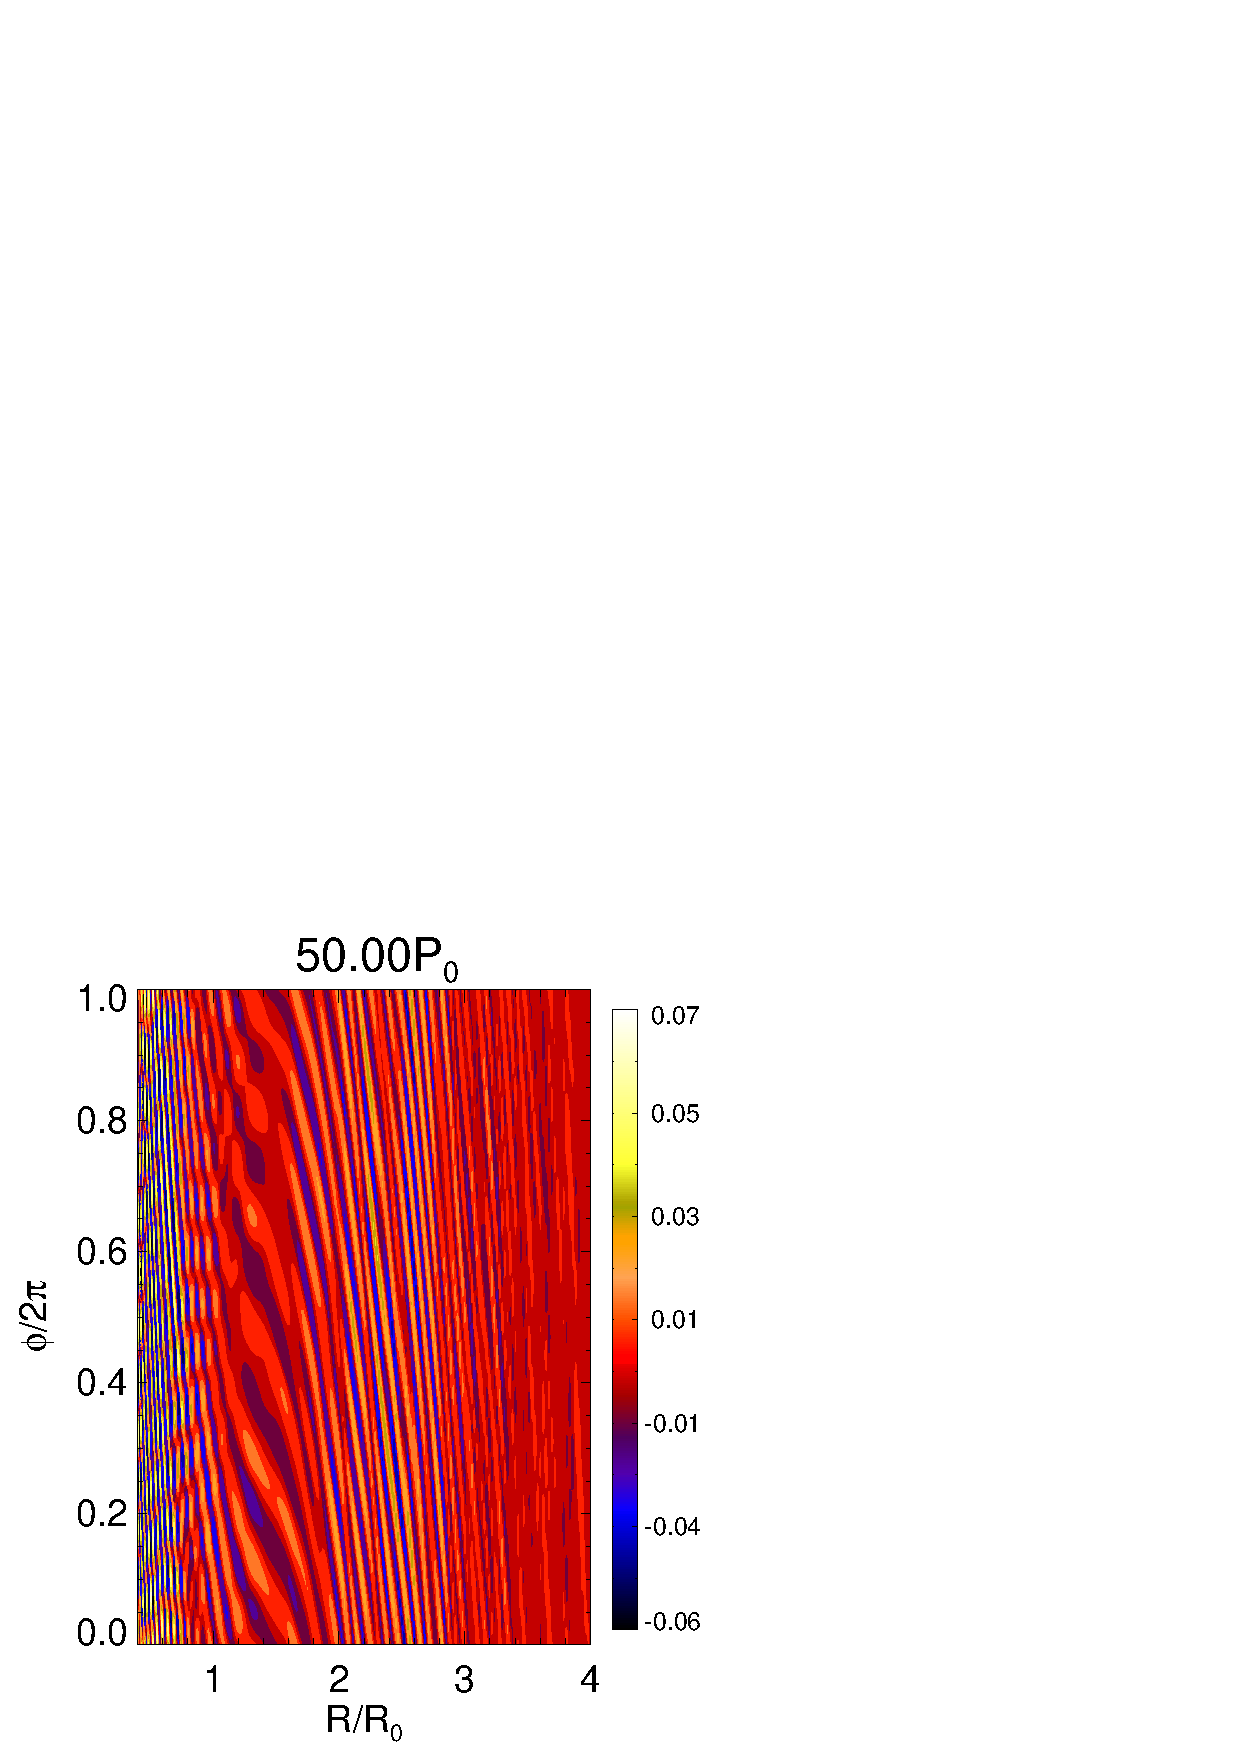
\includegraphics[scale=0.27]{figures/polarxy_dens050}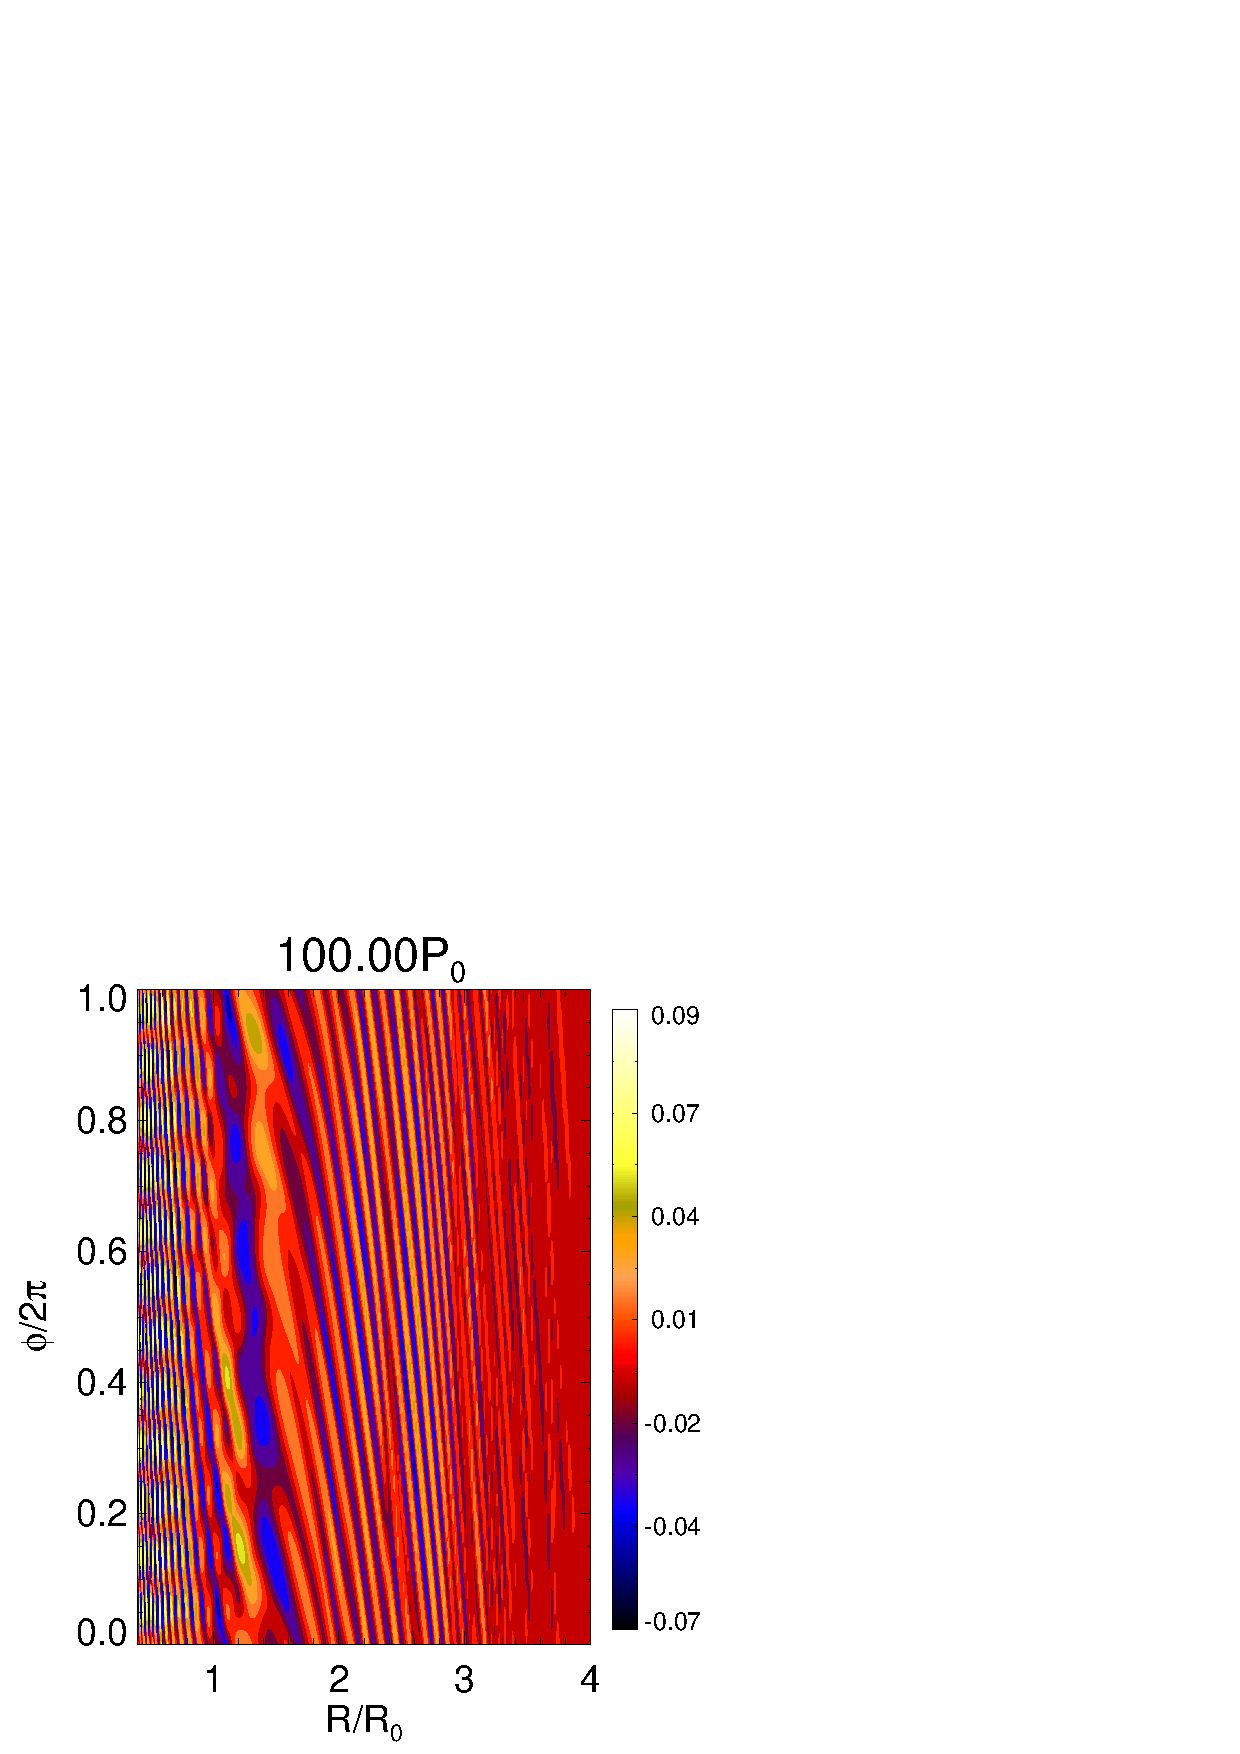
\includegraphics[scale=0.27,clip=true,trim=2.26cm 
  0cm 0cm
  0cm]{figures/polarxy_dens100}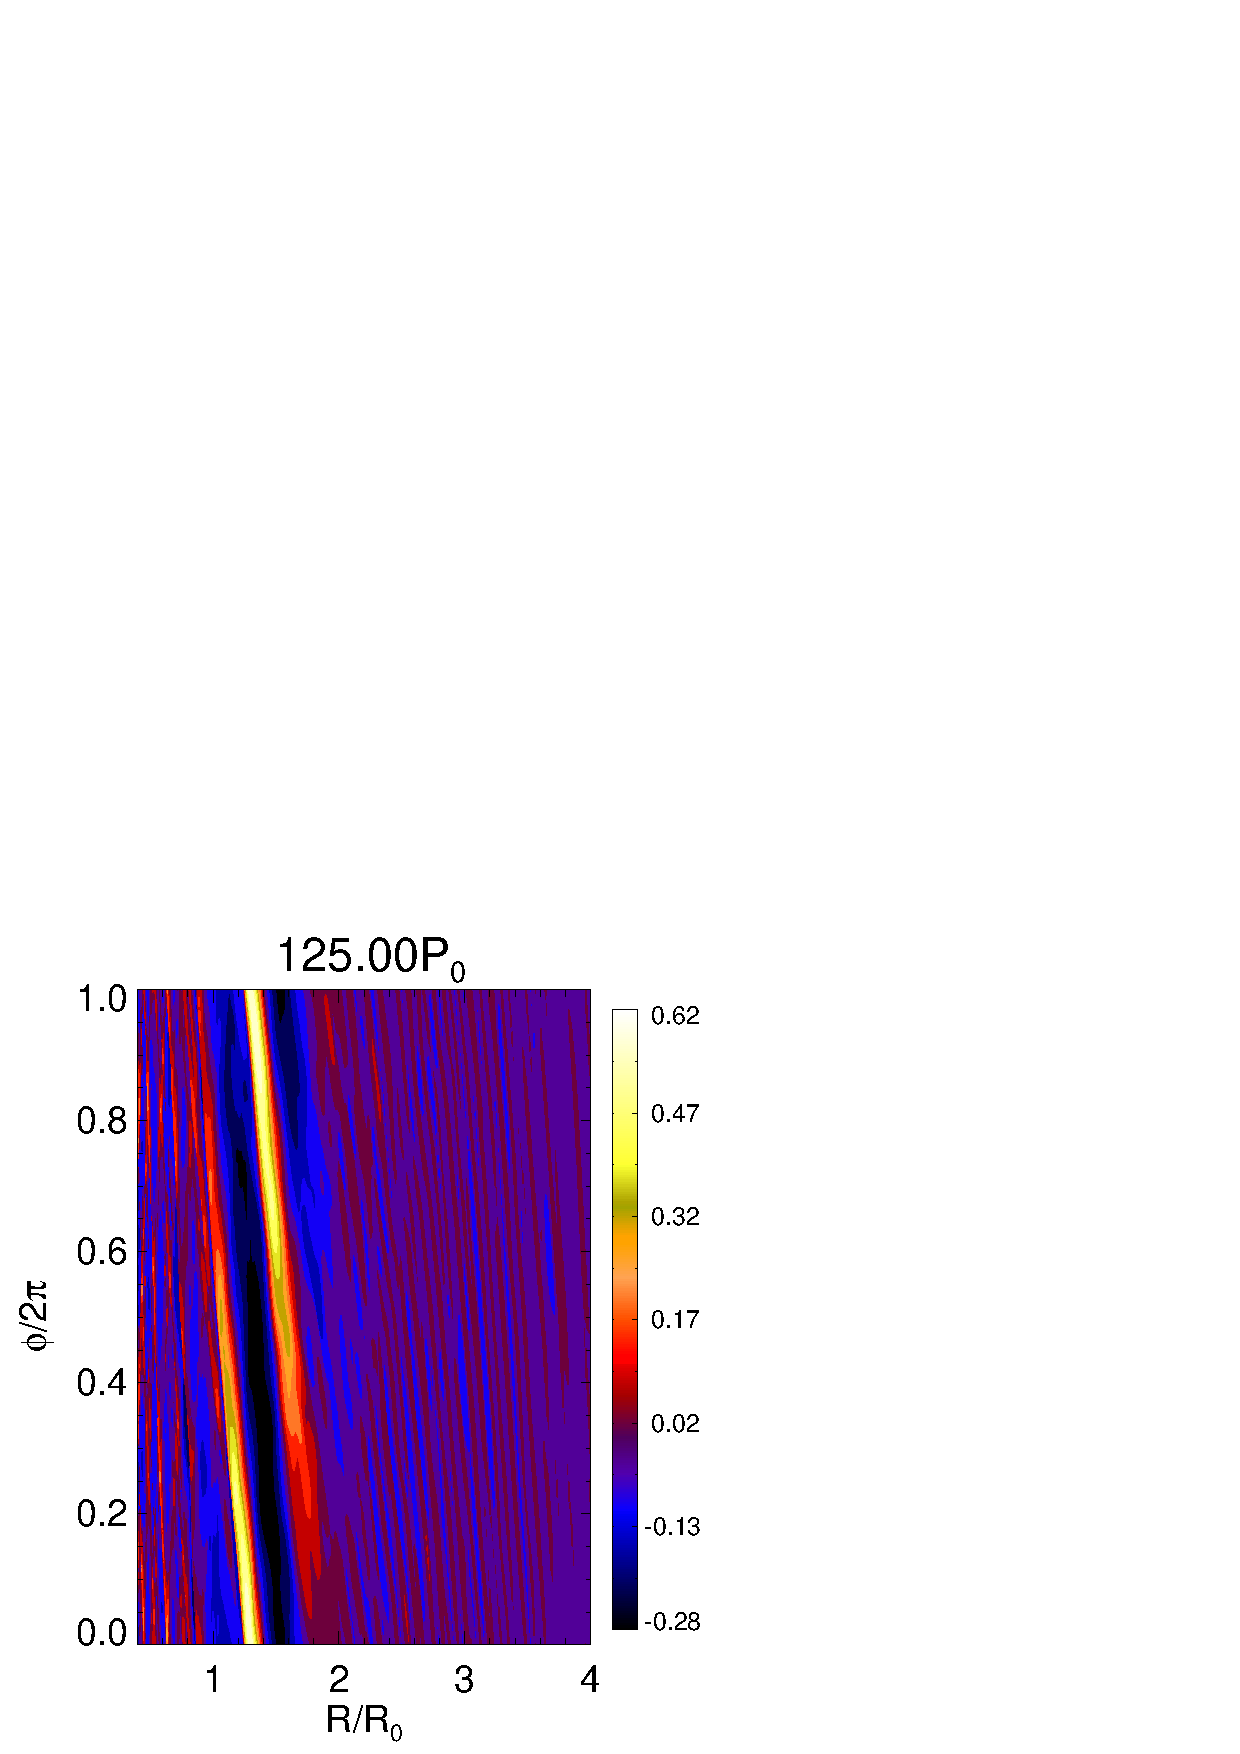
\includegraphics[scale=0.27,clip=true,trim=2.26cm
  0cm 0cm 0cm]{figures/polarxy_dens125} 
  \caption{Preliminary FARGO 2D simulation (\S\ref{fargo_fiducial}),
    showing the evolution of the non-axisymmetric surface density
    $\Delta\Sigma$. Note that the disc extends to $R=10R_0$, but only
    the inner part is shown for clarity. \label{fargo_2d}} 
\end{figure}

\begin{figure}
  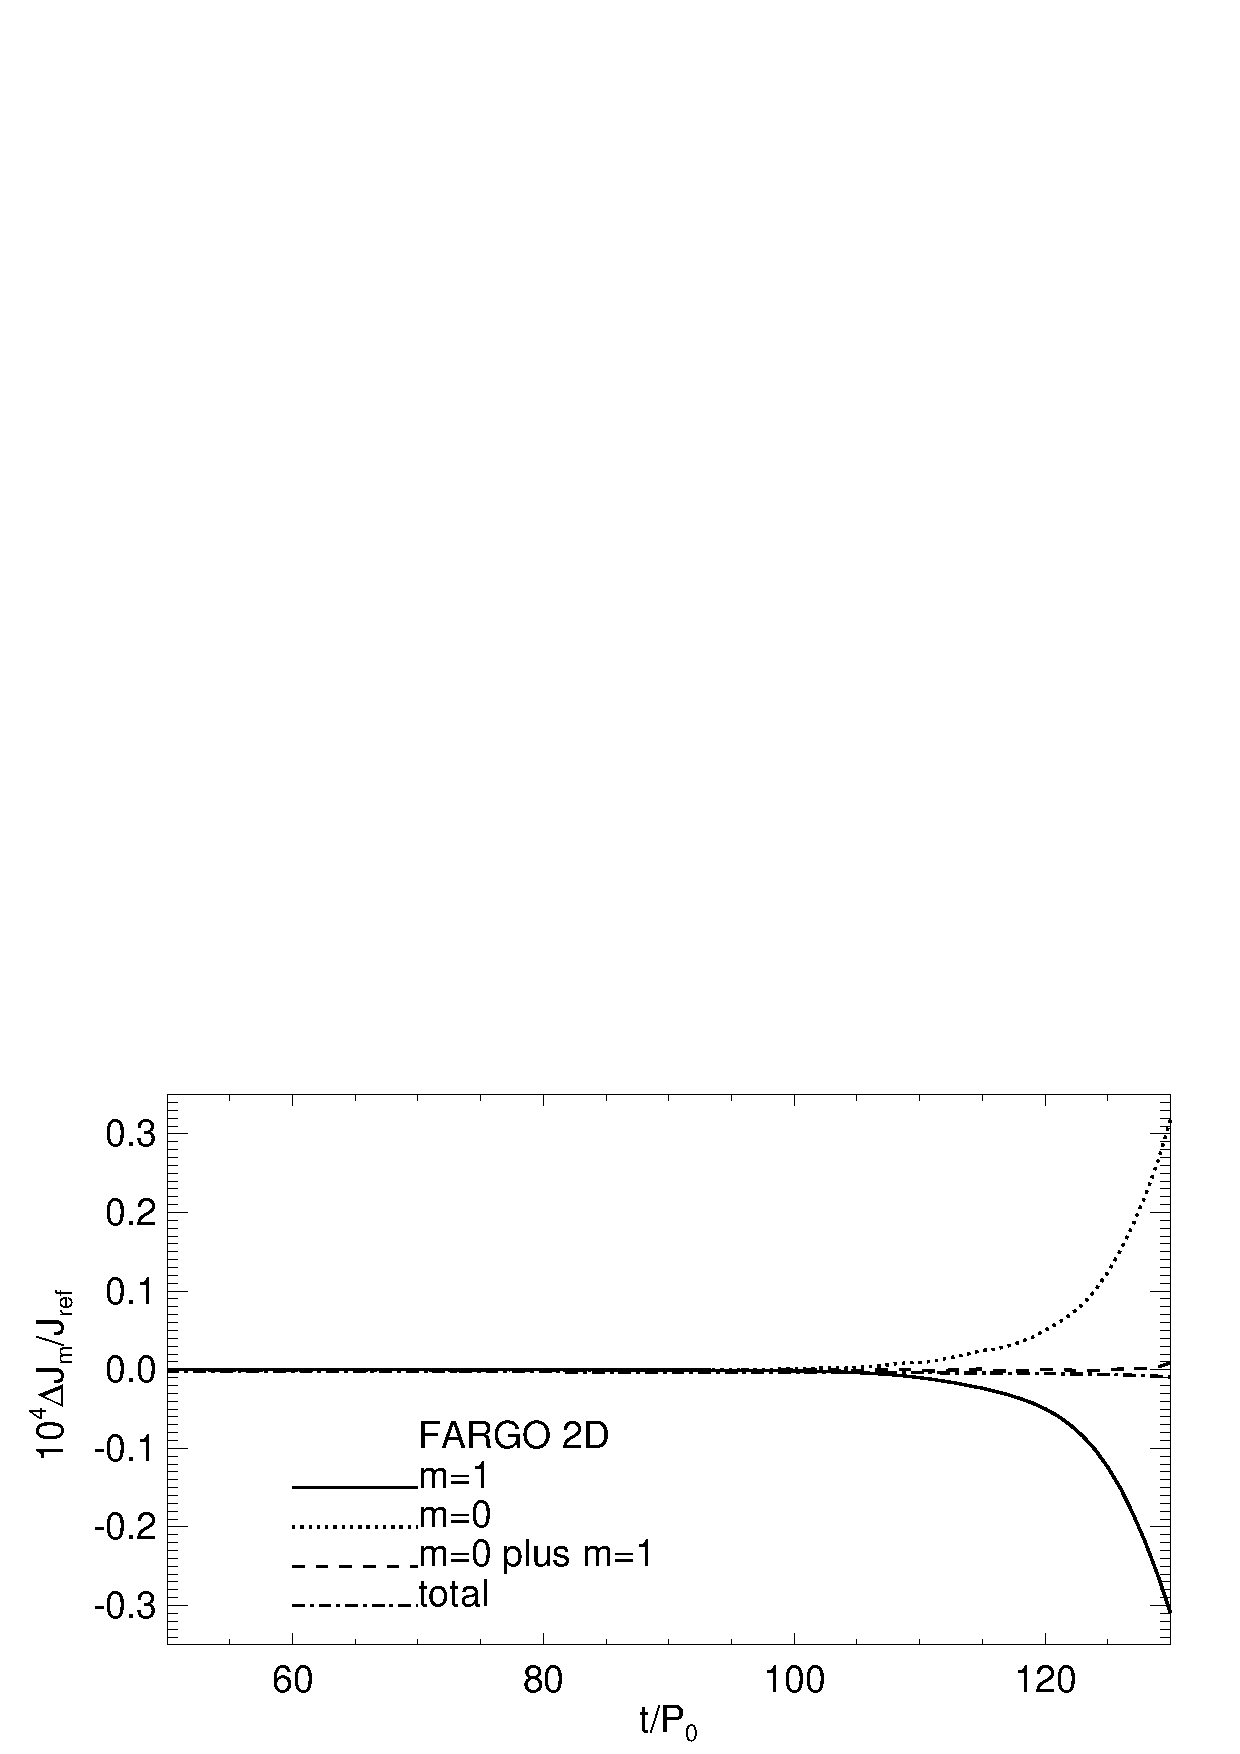
\includegraphics[width=\linewidth]{figures/nonaxi_evol_ang_fargo}
  \caption{Evolution of angular momentum components in the FARGO
     simulation show in Fig. \ref{fargo_2d}. The perturbation
    relative to $t=0$ is shown in units of the initial total angular
    momentum $J_\mathrm{ref}$.\label{fargo_2d_angmom}} 
\end{figure}

\subsection{3D runs}
The 3D disc has radial size 
$[r_\mathrm{min},r_\mathrm{max}]=[0.4,10]R_0$ and vertical extent
$n_H=2$ scale-heights. The resolution is $N_r\times N_\theta\times
N_\phi=256\times32\times256$. Because of the much reduced resolution
compared to 2D, we use a smooth perturbation by setting
$\delta = 10^{-3}$ and $M=1$. This corresponds to a single $m=1$
spiral in the dead zone, which was found to dominate the 2D
simulation. 

Our 3D discs are initialised in approximate equilibrium only, so we
first evolve the disc without perturbations using  
$(\lmax,\mmax)=(32,0)$ up to $t=10P_0$, during which 
meridional velocities are damped out. We then restart the simulation
with the above perturbation and $(\lmax,\mmax)=(32,32)$. 

Snapshots at the end of the simulations are shown in
Fig. \ref{3d_prelim} for both ZEUS-MP and PLUTO. We again
find the dead zone eventually dominated by an $m=1$ spiral. Note that
the amplitude of the spiral is smaller than the 2D case above,
possibily due to lower resolution and/or 3D self-gravity being weaker
than that in 2D. 

\begin{figure}
  \begin{center}
    \subfigure[ZEUS-MP]{
      \includegraphics[scale=0.33]{figures/polarxy_dens015_zeus}
    }
    \subfigure[PLUTO]{
      \includegraphics[scale=0.33]{figures/polarxy_dens015_zeus}
    }
  \end{center}
  \caption{Preliminary 3D simulations using the (a) ZEUS-MP and (b)
    PLUTO. The non-axisymmetric midplane density at the end of the run
    is shown. Here $\psi \equiv \pi/2 - \theta$ is the angular height
    from the midplane.\label{3d_prelim}}   
\end{figure}


Fig. \ref{3d_prelim_angmom} shows the angular momentum evolution in
the 3D runs. ZEUS-MP does not conserve angular momentum very well, but
the variation $|\Delta J/J|< O(10^{-5})$ is not significant compared
to the individual components $|\Delta J_{0,1}/J|\sim
6\times10^{-5}$. We found high-$m$ structures to develop near the
inner boundary, which may have contributed to this error. It
is clear, however, that the growth of negative angluar momentum in
$m=1$ is accompanied by an increase in the background angular
momentum. 

\begin{figure}
  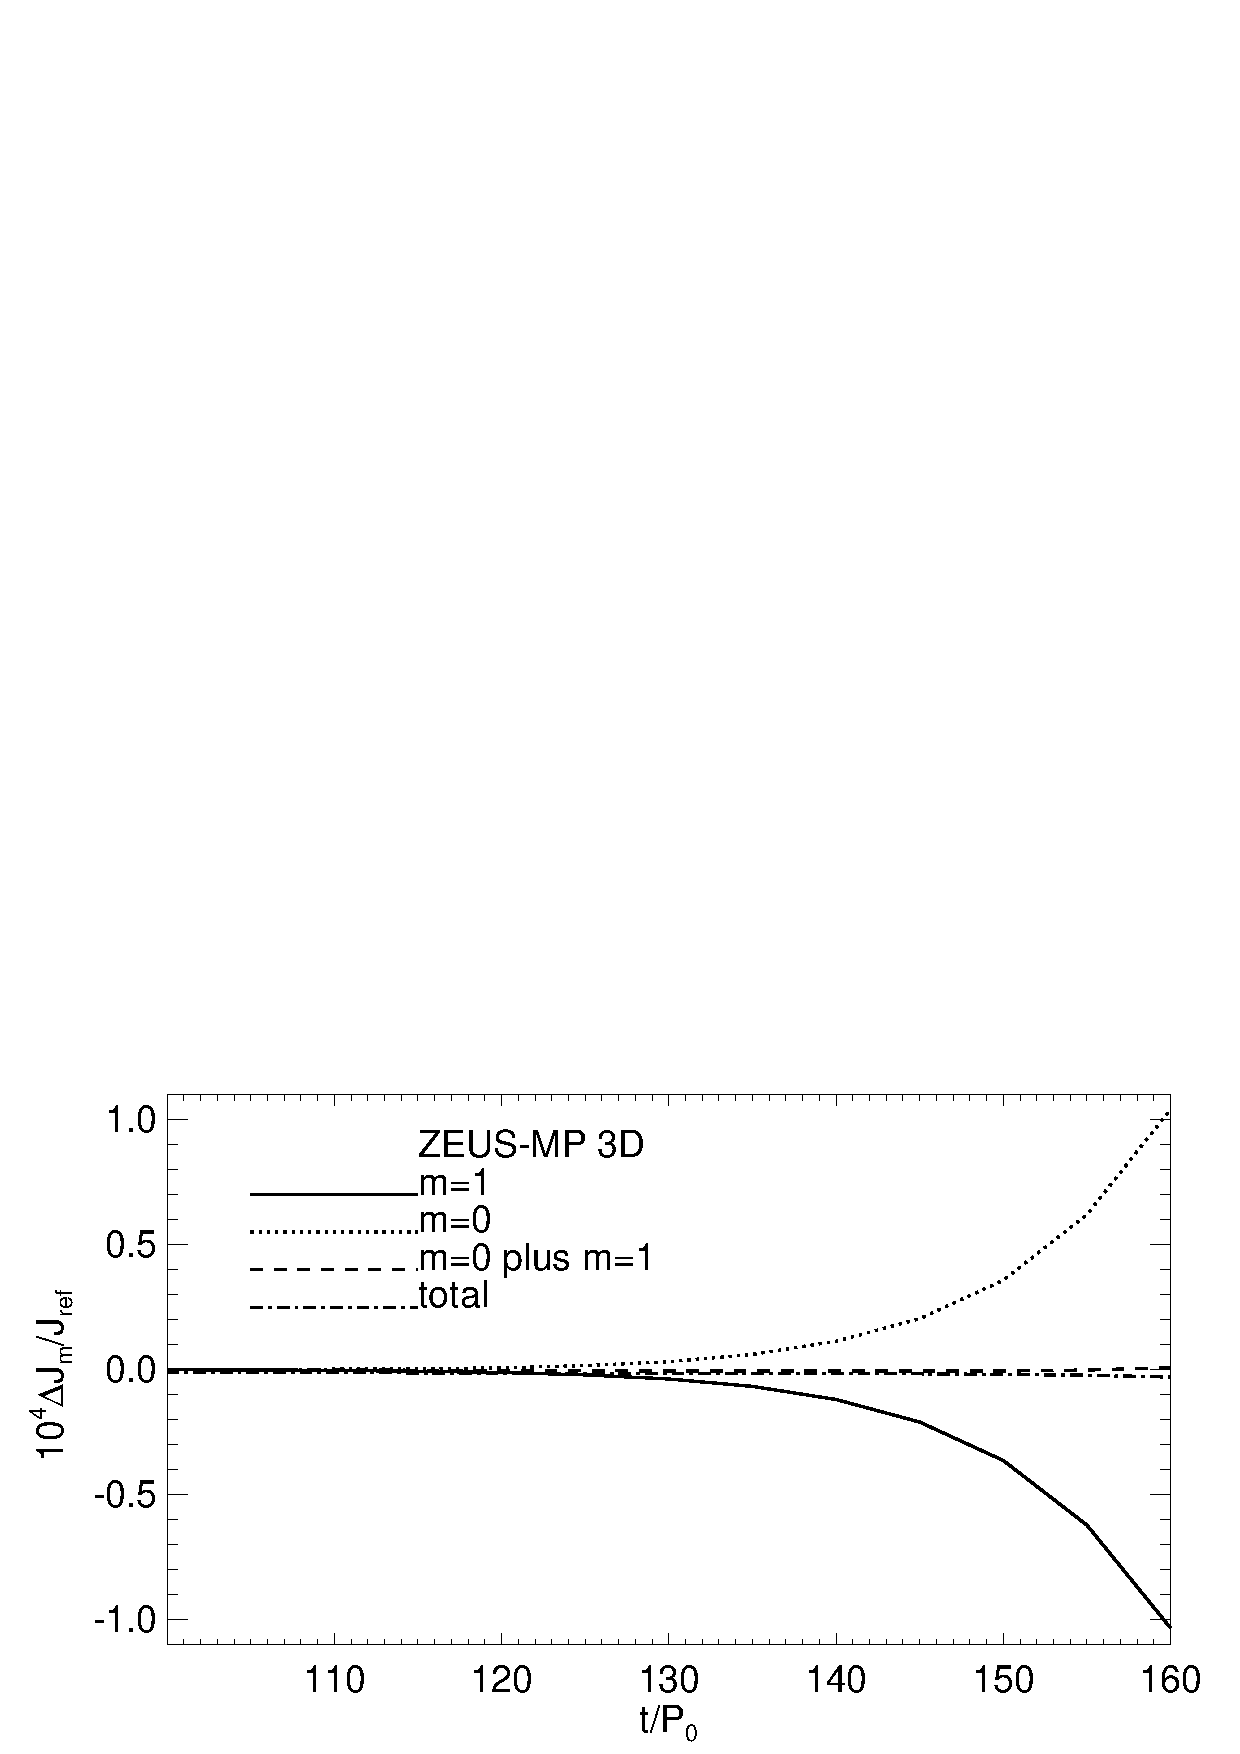
\includegraphics[scale=0.41,clip=true,trim=0cm 1.75cm 0cm 0cm]{figures/nonaxi_evol_ang_zeus}
  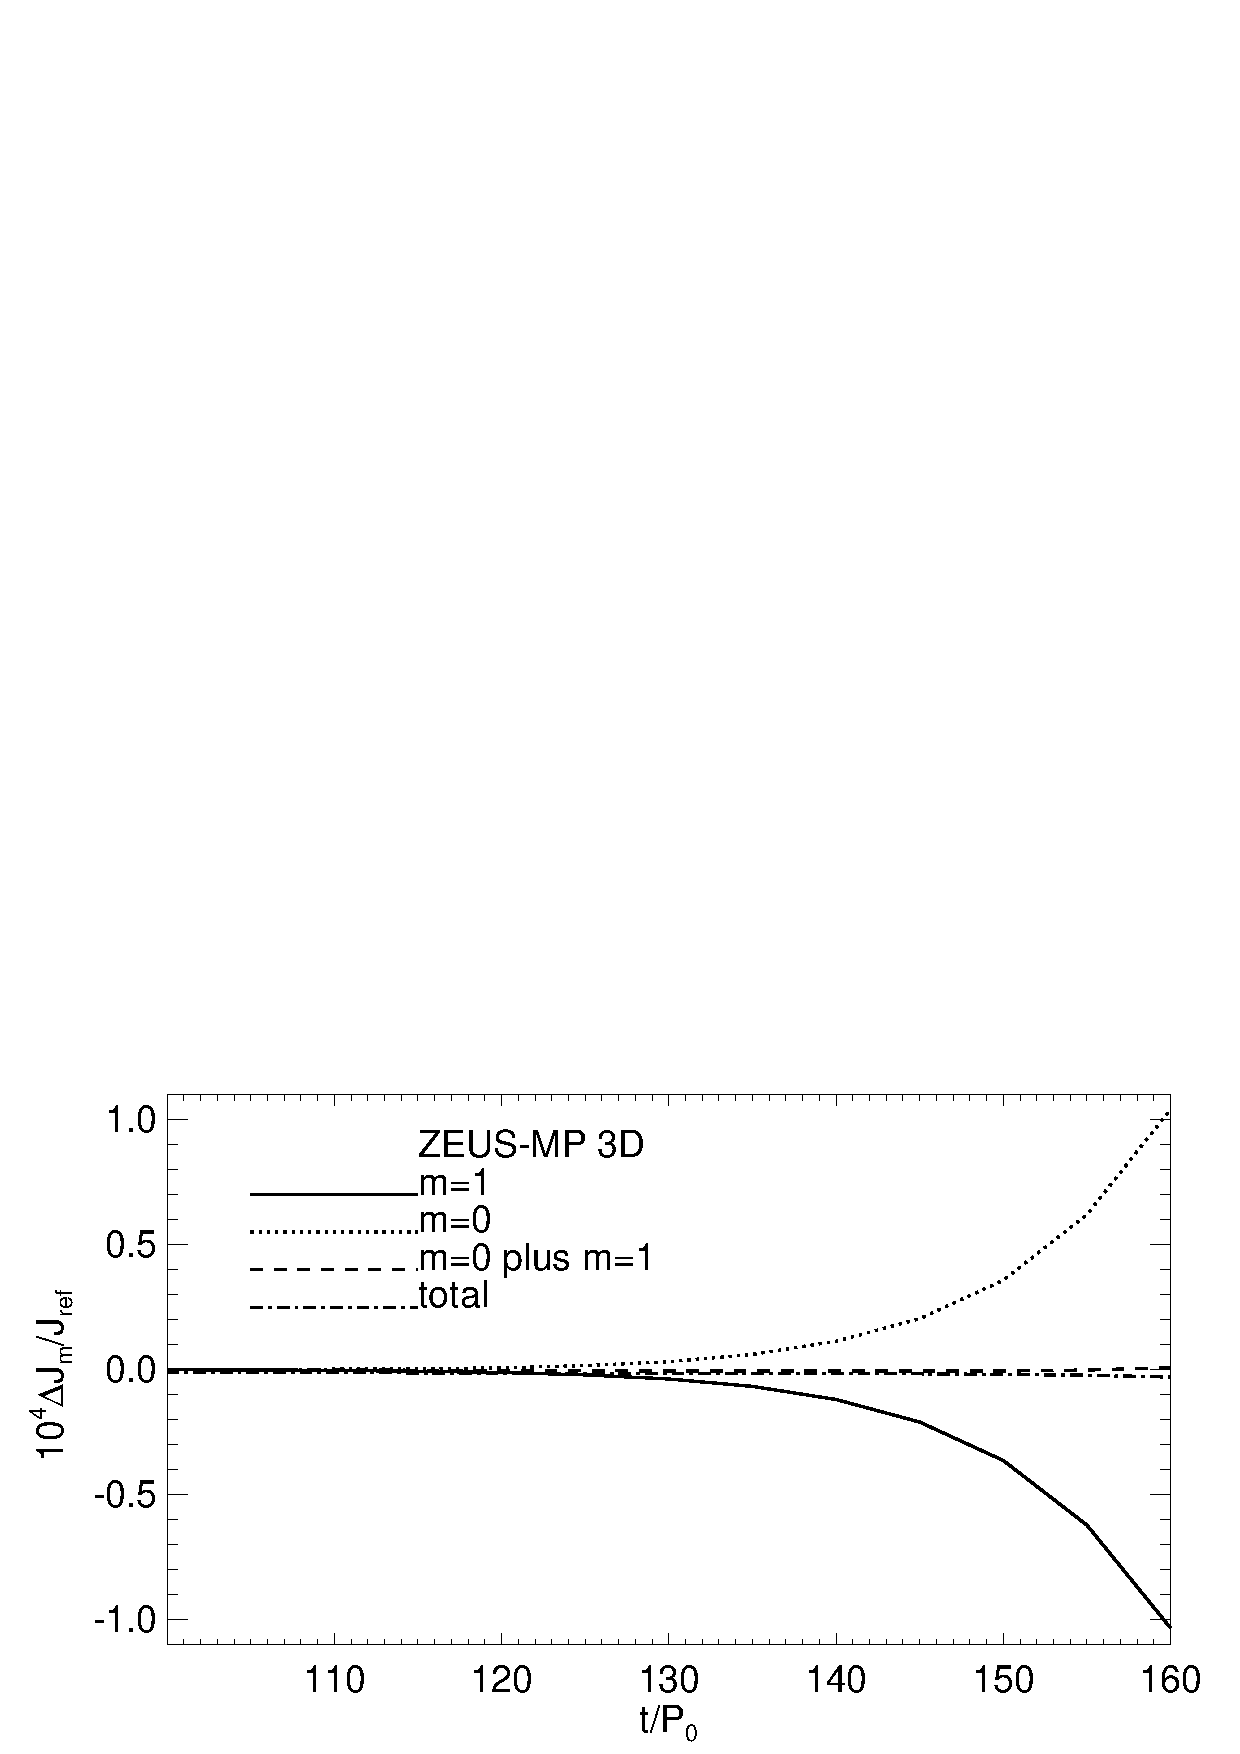
\includegraphics[scale=0.41]{figures/nonaxi_evol_ang_zeus}
  \caption{Evolution of angular momentum components in the 3D 
    simulations show in Fig. \ref{3d_prelim}. The perturbation
    relative to $t=10P_0$ is shown in units of the initial total
    angular momentum $J_\mathrm{ref}$.\label{3d_prelim_angmom}} 
\end{figure}   

\section{Global one-arm spirals in structured discs}

\subsection{Properties of the $m=1$ dead zone spiral}

%\subsection{Three-dimensional structure}

%\section{Additional simulations}
%survery
\section{Three-dimensional simulations}
In this section we briefly review 3D simulations carried 
out using ZEUS-MP and PLUTO. The main purpose is to check 
the above results with different numerical codes, and validate  
the 2D approximation.    

The 3D disc has radial size
$[r_\mathrm{min},r_\mathrm{max}]=[0.4,10]R_0$ and vertical extent 
$n_H=2$ scale-heights. The resolution is $N_r\times N_\theta\times
N_\phi=256\times32\times256$. This corresponds to about $4$ cells per
$H$in radius. 
Because of the much reduced resolution 
compared to 2D, we use a smooth perturbation by setting
$\delta = 10^{-3}$ and $M=1$ in Eq. \ref{randpert}. This corresponds
to a single $m=1$ disturbance in $R\in[R_1,R_2]$, which was found to dominate
the 2D simulation.  

Our 3D discs are initialised in approximate equilibrium only, so we
first evolve the disc without perturbations using  
$(\lmax,\mmax)=(32,0)$ up to $t=100P_0$, during which 
meridional velocities are damped out. We then restart the simulation
with the above perturbation and $(\lmax,\mmax)=(32,32)$. 


Fig. \ref{3d_ampmax} plots the amplitude of the $m=1$ spirals measured
in the ZEUS-MP and PLUTO runs. We also show results from strictly
isothermal discs ($q=0$), which clearly display no growth. %why no high m
                                %modes as in 2D for iso disc?
                                %resolution?
Results from ZEUS-MP appears to be off-set from that obtained using
PLUTO. We suspect this may be due to larger numerical noise in the
ZEUS-MP code. Thus the $m=1$ spiral grows to a larger amplitude by the
end of the run. However, we measure similar growth rates,
\begin{align*}
&\gamma \simeq 0.0073\Omega_k(R_0) \quad\quad \mathrm{PLUTO},\\
&\gamma \simeq 0.0075\Omega_k(R_0) \quad\quad \mathrm{ZEUS-MP}.
\end{align*}
Both are smaller than the 2D simulations above. This may be due to the
low resolutions adopted. 
%growth rate does not depend on pert amp

\begin{figure}
  \includegraphics[width=\linewidth]{figures/m1_analysis_plot_ampmax3d.ps}
  \caption{Evolution of the maximum $m=1$ density in  $r\in[R_1,R_2]$
    measured in the 3D simulations. Both discs with a imposed
    temperature gradient ($q=1$) and a strictly isothermal disc
    ($q=0$) are shown. 
    \label{3d_ampmax}}   
\end{figure}

Visualisations of the 3D simluations are shown in Fig. \ref{3d_prelim} for
both ZEUS-MP and PLUTO. The snapshots are chosen for when the spiral
amplitudes are similar. The agreement between the two codes, as well
as with the 2D simulations, is satisfactory. 

%but a longer PLUTO simulation was 
%needed to achieve similar mode amplitudes in ZEUS-MP. 


\begin{figure}
  \begin{center}
    \subfigure[ZEUS-MP]{
      \includegraphics[scale=0.33]{figures/polarxy_dens015_zeus}
    }
    \subfigure[PLUTO]{
      \includegraphics[scale=0.33]{figures/pdisk_020}
    }
  \end{center}
  \caption{Three-dimensional simulations using the (a) ZEUS-MP and (b)
    PLUTO. The non-axisymmetric midplane density is shown. Here $\psi
    \equiv \pi/2 - \theta$ is the angular height 
    from the midplane.\label{3d_prelim}}   
\end{figure}

\subsection{Vertical motion}

\subsection{Angular momentum evolution}

Fig. \ref{3d_angmom} shows the angular momentum evolution in the 3D
runs. ZEUS-MP does not conserve angular momentum very well, but
the variation $|\Delta J/J|< O(10^{-5})$ is not significant compared
to the individual components $|\Delta J_{0,1}/J|\sim 
6\times10^{-5}$. The PLUTO run reaches similar values of
$|J_{0,1}|$, but achieves better conervation, with $|\Delta
J/J|=O(10^{-8})$. 



\begin{figure}
%scale=0.41
  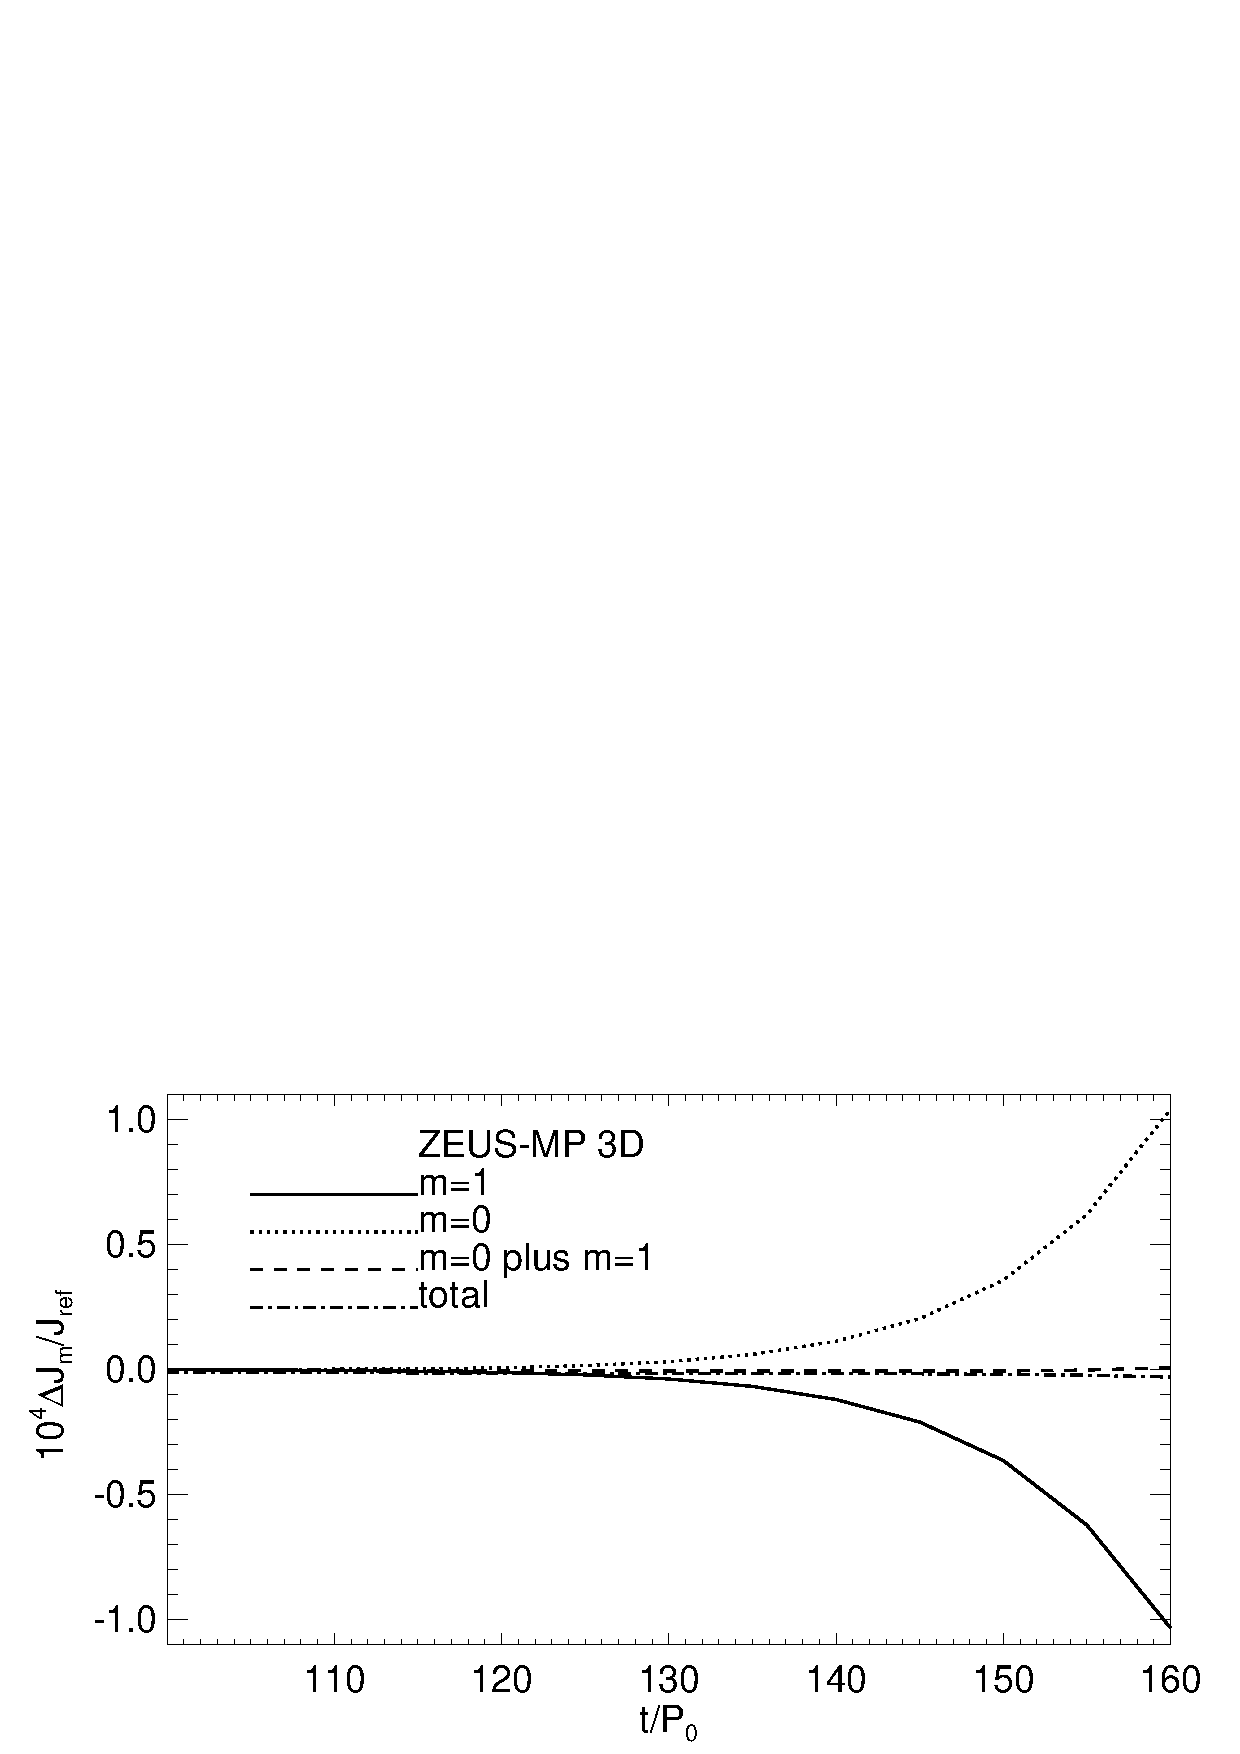
\includegraphics[scale=.41,clip=true,trim=0cm 1cm 0cm 0cm]{figures/nonaxi_evol_ang_zeus}
  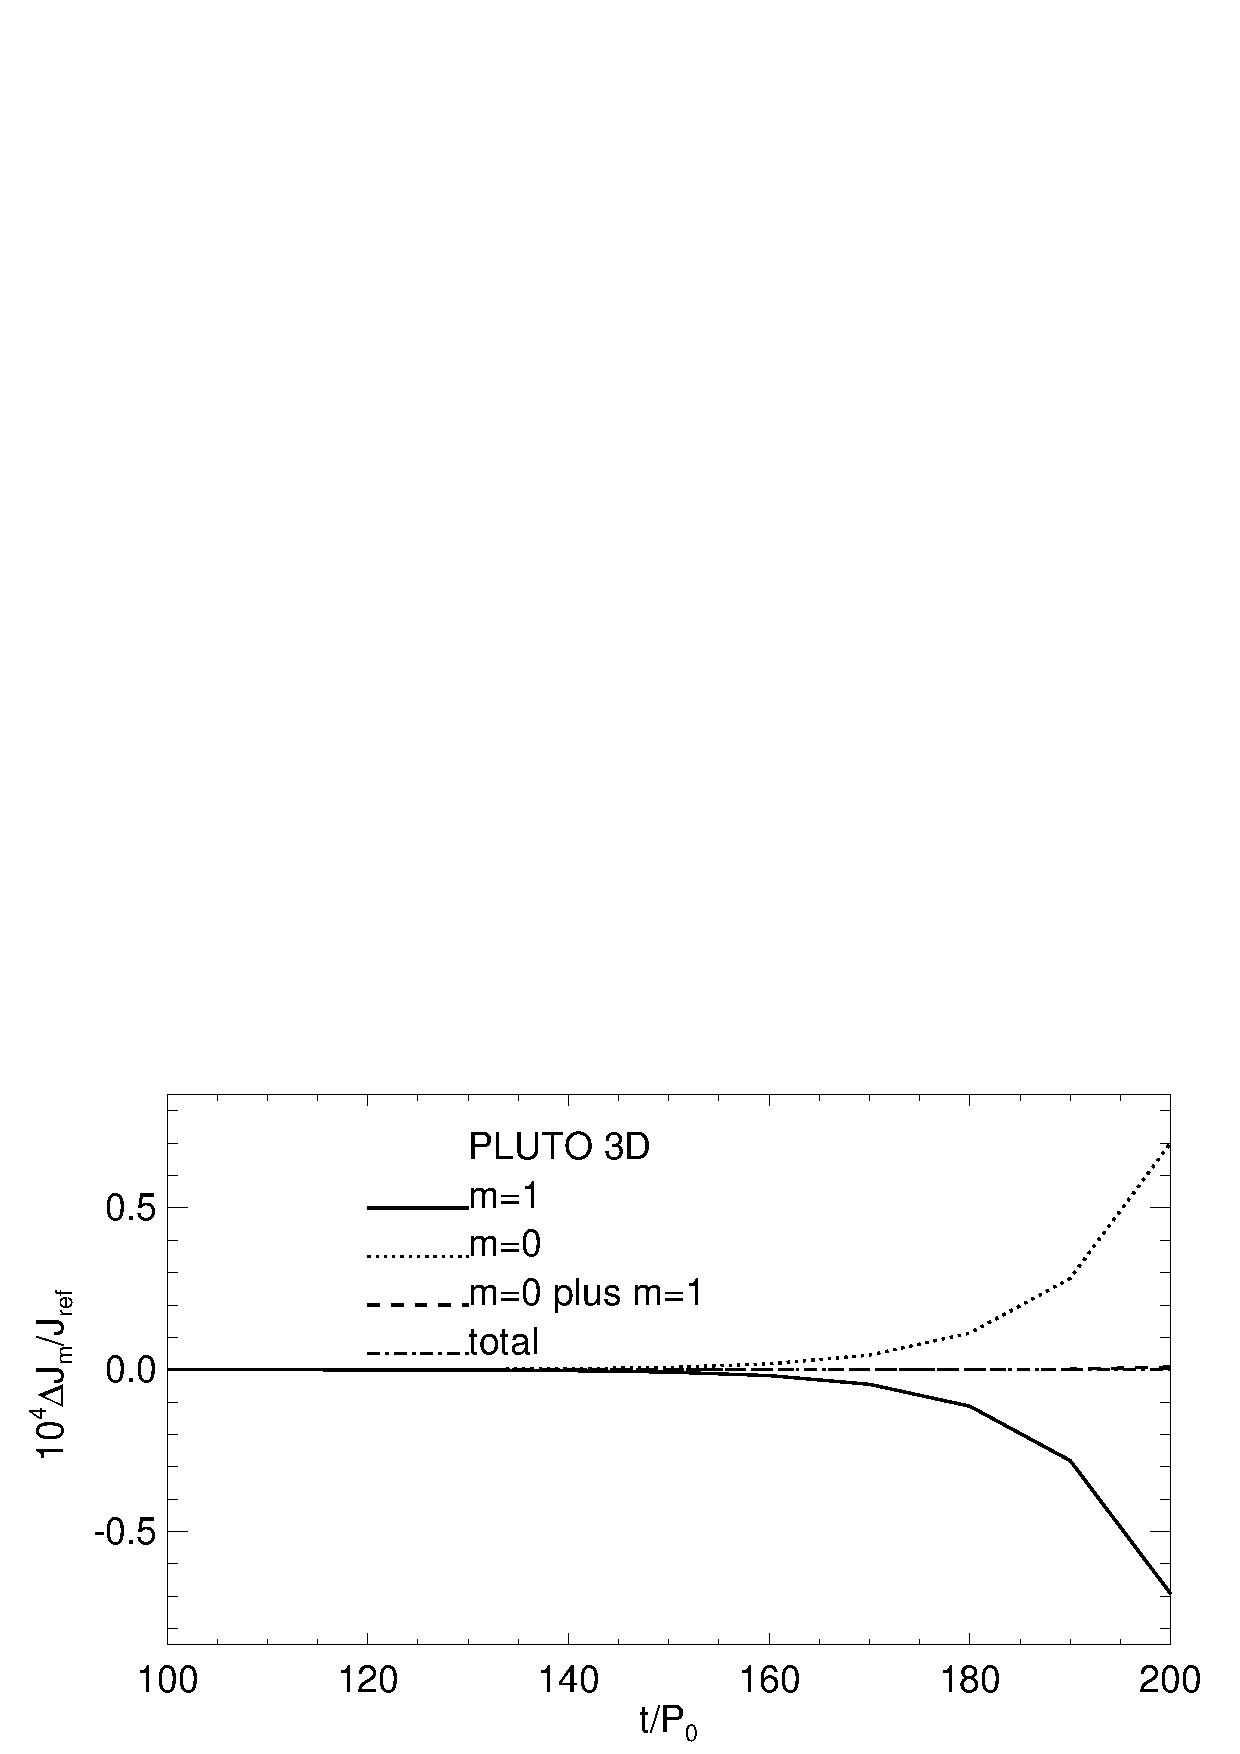
\includegraphics[scale=.41]{figures/nonaxi_evol_ang_pluto}
  \caption{Evolution of angular momentum components in the fiducial 3D 
    simulations. The perturbation
    relative to $t=100P_0$ is shown in units of the
    initial total angular momentum $J_\mathrm{ref}$.\label{3d_angmom}} 
\end{figure}   


\section{Discussion}
Having confirmed the $m=1$ spiral instability through numerical
simulations, we now use results from the simulations combined with
linear theory to construct an explanation for their growth. For
simplicitly, we return to 2D discs. 

\subsection{Angular momentum density of  low-frequency $m=1$ modes}
From Eq. \ref{lin_ang_mom_cons} and assuming a time-dependence of the
form $\exp{(-\ii \sigma t)}$ with $\real{\sigma} = \omega$,  
the angular momentum density associated with linear waves is
\begin{align}
  \jlin = \frac{m\Sigma}{2}\left[\left(\omega -
      m\Omega\right)|\bm{\xi}|^2 + \ii\Omega\left(\xi_R\xi_\phi^* -
      \xi_R\xi_\phi^*\right)\right].  
\end{align}
For a low-frequency mode, $|\omega|\ll m\Omega$. Then neglecting the
term $\omega|\bm{\xi}|^2$ and setting $m=1$,
\begin{align}
  \jlin &\simeq \frac{\Sigma\Omega}{2}\left[-|\bm{\xi}|^2 + \ii\left(\xi_R\xi_\phi^* -
      \xi_R\xi_\phi^*\right)\right]\notag\\
  & = -\frac{\Sigma\Omega}{2}|\xi_R + \ii\xi_\phi|^2\notag\\
  & \leq 0.
\end{align}
Thus, low-frequency $m=1$ modes are generally associated with negative
angular momentum. If the mode loses (positive) angular momentum
to the background, then we can expect instability. We demonstrate
this below. 

\subsection{Unstable interaction between low-frequency $m=1$ spirals
  and the background disc due to an imposed temperature gradient}
The $m=1$ spiral that emerges in our simulations have low frequency
and grows slowly, and its spatial form is consistent local theory
(\S\ref{fargo_m1}). To demonstrate possible instability, we
first construct a neutral low-frequency mode using local theory, then
show that the torque density acting on this mode due to the background
temperature gradient is negative, which enforces the mode. % Note that
% we will not be assuming a self-gravitating disc until the end of this
% section. 

We begin by recalling the expression for the torque density due to a
locally isothermal equation of state,
\begin{align}
  T_\mathrm{BG} &= -\frac{m}{2}\frac{dc_s^2}{dR}\imag\left[\delta\Sigma_m \left(\frac{\delta
        v_{Rm}}{-\ii\sbar}\right)^*\right] \notag\\
  & = \frac{m}{2}\frac{dc_s^2}{dR}\imag\left[\ii \delta\Sigma_m \left(\frac{\delta
        v_{Rm}}{\sbar}\right)^*\right]
\end{align}
where we replaced the radial Lagrangian displacement by the Eulerian
radial velocity perturbation in Eq. \ref{baroclinic_torque}. 
The linearised momentum equations give
\begin{align}
  D\delta v_{Rm} =& 
  \ii\sbar\left[c_s^2\frac{d}{dR}\left(\frac{\delta\Sigma_m}{\Sigma}\right)
    + \frac{d}{dR}\delta\Phi_m\right] \notag\\ 
  &- \frac{2\ii
    m\Omega}{R}\left(c_s^2\frac{\delta\Sigma_m}{\Sigma} +
    \delta\Phi_m\right),
\end{align}
where $D\equiv \kappa^2 - \sbar^2$. 

We now invoke local theory by setting $d/dR \to \ii k$ where $k$ is
real, and using the local solution to the Poisson equation
\begin{align}
  \delta\Phi_m = -\frac{2\pi G}{|k|}\delta\Sigma_m 
\end{align}
\citep{shu91}. Then the radial velocity perturbation becomes
\begin{align}
  \delta v_{Rm} =
  \frac{1}{D}\frac{\delta\Sigma_m}{\Sigma}\left(\frac{2\pi G
      \Sigma}{|k|} - c_s^2\right)\left(k\sbar + \frac{2\ii
      m\Omega}{R}\right),
\end{align}
so that 
\begin{align}
  \ii\delta\Sigma_m \left(\frac{\delta v_{Rm}}{\sbar}\right)^* =
  \frac{1}{D^*}\frac{|\delta\Sigma_m|^2}{\Sigma}\left(\frac{2\pi G
      \Sigma}{|k|} - c_s^2\right)\left(\ii k  + \frac{2
      m\Omega}{R\sbar^*}\right). 
\end{align}
For a neutral mode, $\sbar$, and therfore $D$ is real. Then, after
taking the imaginary part of the above expression, the torque
density is 
\begin{align}\label{tbg_explicit}
  T_\mathrm{BG} &=
  \frac{m}{2}\frac{dc_s^2}{dR}\left[\frac{k}{D}\frac{|\delta\Sigma_m|^2}{\Sigma}\left(\frac{2\pi G
      \Sigma}{|k|} - c_s^2\right)\right].
% &\simeq \frac{m}{2}\frac{dc_s^2}{dR}\left[\frac{k}{\left(\kappa^2 -
%         m^2\Omega^2\right)}\frac{|\delta\Sigma_m|^2}{\Sigma}\left(\frac{2\pi
%       G \Sigma}{|k|} - c_s^2\right)\right]. 
\end{align}
%where the second line follows from the low-frequency approximation
%$|\sigma|\ll m\Omega$. 
% To determine the sign of $T_\mathrm{BG}$ for low frequency one-arm spirals,
% we examine each factor separately below for $m=1$:
% \begin{itemize}
% \item We observe trailing spirals in our simulations, so $k>0$. 
% \item The factor $\kappa^2 - \Omega^2>0$ for our self-gravitating disc
%   models in the region where the spiral appears. 
% \item We measure $|k|\sim \pi G\Sigma/c_s^2$, so the last factor in
%   the square brackets is positive. Note that this factor is positive
%   provided $|k| < 2/HQ$ or wavelengths $\lambda > \pi Q H$.  
% \end{itemize}
We now use the local dispersion relation,
Eq. \ref{dispersion}, to make the replacement $D = 2\pi G \Sigma |k| -
k^2c_s^2$ in the above expression. This gives
\begin{align}\label{tbg_simple}
  T_\mathrm{BG} =
  \frac{m}{2}\frac{dc_s^2}{dR}\frac{1}{k}\frac{|\delta\Sigma_m|^2}{\Sigma}.  
\end{align} 
This torque density is negative for trailing waves in discs with
temperature decreasing outwards ($k>0$ and $dc_s^2/dR<0$,
respectively). Note that this conclusion does not rely on the
low-frequency approximation and holds for any $m$.   

However, if the linear disturbance under consideration \emph{is} a
low-frequency $m=1$ 
trailing spiral wave, then it has negative angular
momentum. If $dc_s^2/dR<0$, as is typical for circumstellar or
protoplanetary discs, then $T_\mathrm{BG}<0$, and the background disc
applies a negative torque on the disturbance, which further decreases
its angular momentum. This suggests the spiral amplitude will grow.  


Using $\jlin$ and $T_\mathrm{BG}$, we can obtain a rough estimate of
the growth rate $\gamma$ of linear perturbations as  
\begin{align}
  2\gamma \sim \frac{T_\mathrm{BG}}{\jlin},
\end{align}
where the factor of two accounts for the fact that the angular momentum
density is quadradtic in the linear perturbations. Inserting the above
expressions for $\jlin$ and $T_\mathrm{BG}$ for $m=1$ gives
\begin{align}
  2\gamma \sim
  -\frac{dc_s^2}{dR}\frac{1}{k\Sigma^2\Omega}\frac{|\delta\Sigma_1|^2}{|\xi_R
    + \ii\xi_\phi|^2}.
\end{align}
Now, using $\delta\Sigma_m/\Sigma = -\ii k \xi_R - \ii m \xi_\phi/R$
in the local approximation, we have
\begin{align}
  2\gamma \sim -\frac{dc_s^2}{dR}\frac{k}{\Omega}\frac{|\xi_R +
    \xi_\phi/kR|^2}{|\xi_R + \ii \xi_\phi|^2}
  \lesssim -\frac{dc_s^2}{dR}\frac{k}{\Omega}.
\end{align}
where we used $dc_s^2/dR <0$, $k>0$ and $|kR|\gg 1$ to obtain the
inequality. For $c_s^2 = c_{s0}^2 (R/R_0)^{-q}$ adopted in our disc
models,
\begin{align}\label{theoretical_rate}
  2\gamma \lesssim q\frac{c_s^2}{R}\frac{k}{\Omega}. 
\end{align}
Now we consider perturbations in a self-gravitating disc with characteristic
wavenumber $k \sim \pi G \Sigma/c_s^2 \sim \Omega/Q c_s$ (as seen in
our simulations). Then
\begin{align}
  \gamma \lesssim \frac{qh}{2Q}\Omega,
\end{align}
where we used $c_s/R\sim h\Omega$. For our fiducial disc models with
$q=1$, $Q=O(1)$, $h=0.05$, this gives $\gamma/\Omega = O(10^{-2})$,
consistent with simulation results. 

Of course, we have been assuming a neutral mode to obtain expressions
for $\jlin$ and $T_\mathrm{BG}$ in the first place, so
Eq. \ref{theoretical_rate} is only an order-of-magnitude
constraint. Nevertheless, the xpected growth rate is in reasonable
agreement with numerical results. 

%also total torque is integral -> may get cancelations 

\subsection{Role of self-gravity and disc structure} 
We note that the background torque density $T_\mathrm{BG}$ does not depend on  
self-gravity, and we only considered a self-gravitating perturbation to
obtain an appropriate wavenumber $k$ needed to evaluate
Eq. \ref{theoretical_rate}. Thus, self-gravity is not directly
responsible for instability. However, 
our numerical simulations show that the $m=1$ spiral is
confined between two $Q$-barriers, where real solutions to the local
dispersion relation is possible (Eq. \ref{wavenumber}), as a result of the adopted disc
structure. Thus, the main role of disc structure and self-gravity is to
allow a neutral mode to be set up and confined, which is then
destabilised through the background torque density. 

%talk about additional simulations at high Q
%spiral mode as external potential to wider disc (lp11)
%interaction across co-rotation

\subsubsection{The confined spiral as an external potential}
One possible effect of self-gravity is to allow the one-arm spiral 
to act as an external potential for the wider disc. This effect is
analogous to disc-satellite interaction 
\citep{goldreich79}, and may lead to instability 
if the angular momentum associated with the spiral has the opposite 
sign to that of the density waves it induces in the exterior disc
\citep{lin11b}. To estimate this effect, we port basic results from
disc-planet theory \citep[see, e.g.][and references
therein]{papaloizou07}. 

Let us regard the one-arm spiral disturbance located in the inner disc as an  
external potential of the form $\Phi_\mathrm{ext}(R)\cos{\left(\phi -
    \Omega_pt\right)}$. We expect
it to exert a torque on the exterior disc at Lindblad  
and co-rotation resonances. At the outer Lindblad resonance (OLR), this
torque is 
\begin{align}
  \Gamma_L =
  \frac{\pi^2\Sigma_L}{3\Omega_L\Omega_p}
\left[\left.R_L\frac{d\Phi_\mathrm{ext}}{dR}\right|_L + 2\left(1 - \frac{\Omega_p}{\Omega_L}\right)\Phi_\mathrm{ext}\right]^2,
\end{align}   
where a Keperian disc has been assumed and subscript $L$ denotes
evaluation at $R=R_L$. (The inner Lindblad resonance does not exist
for the pattern speeds observed in our simulations.)

To order-of-magnitude, we reasonably take
\begin{align}
  \Phi_\mathrm{ext} = -\frac{GM_\mathrm{ring}}{|R - \bar{R}|}, 
\end{align}
for the potential associated with a disturbance located at
$R=\bar{R}$, where $M_\mathrm{ring}$ is the mass in $R\in[R_1,R_2]$.
If we also associate its angular momentum with 
$J_\mathrm{ext}  = M_\mathrm{ring}\bar{R}^2\Omega_p$, we can obtain a
rate $\gamma_L$ by evaluating $\Gamma_L/J_\mathrm{ext}$. Then 
\begin{align}
  \frac{\gamma_L}{\Omega_p} \sim &\frac{\pi h}{3
    Q_L}\left(\frac{M_\mathrm{ring}}{M_*}\right)\left(\frac{R_L}{\bar{R}}\right)^{-1/2}\left(\frac{R_c}{\bar{R}}\right)^{5/2}\notag\\
  &\times \left\{ \frac{R_L}{R_L - \bar{R}} - 2\left[1 -
      \left(\frac{R_c}{R_L}\right)^{-3/2}\right]\right\}^2\frac{R_c^2}{\left(R_L
    - \bar{R}\right)^2}. 
\end{align}
Inserting $h=0.05$, $Q_L=10$, $M_\mathrm{ring} = 0.05M_*$,
$R_L=7.2R_0$, $R_c=4.4R_0$ and $\bar{R}=1.5R_0$ from our fiducial
FARGO simulation, we get
\begin{align}
  \gamma_L \sim 0.012\Omega_p. 
\end{align}
This represents an upper limit on the effect of the OLR on the spiral
disturbance, and is much smaller than the growth rate measured in the
simulation ($\gamma\sim0.1\Omega_p$). We conclude that for our models,
the OLR has negligible effect on the one-arm spiral. 

For the co-rotation torque, we use the result
\begin{align}
  \Gamma_C = \left.
    \pi^2\Phi_\mathrm{ext}^2\left(\frac{d\Omega}{dR}\right)^{-1}\frac{d}{dR}\left(\frac{2\Sigma}{\Omega}\right)\right|_{C}
\end{align}
for a Keplerian disc, where subscript $C$ denotes evaluation at
co-rotation radius $R=R_c$. For a power-law surface density profile
$\Sigma\propto R^{-s}$ we have
\begin{align}
  \frac{\Gamma_C}{J_\mathrm{ext}\Omega_p} = \frac{4}{3}\frac{\pi h}{Q_C} \left(s -
    \frac{3}{2}\right)\left(\frac{M_\mathrm{ring}}{M_*}\right)\frac{R_c^4}{\bar{R}^2\left(R_c
      - \bar{R}\right)^2}.   
\end{align}
Using the above parameter values with $s=2$ and $Q_c=10$, we obtain a
rate
\begin{align}
  \gamma_C\sim 0.010\Omega_p,
\end{align}
which is again small compared to the measured growth rates. 

%expressions for linear response, but have massive "planet" -> but CR
%and LR far from where spiral is 


%required disc structure (for confined SG spiral)

%\subsection{Speculations}
%speculations - long term balance. forced temp gradient drives
%instability (disc gains ang mom, spiral loses ang mom). but if spiral
%shocks and dissiple, it dumps negative angular momentum (disc gains
%negative ang mom). balance between gain from forced temp gradient and
%loss due to dissiplatoin

%other source of m=1 disturbance -> eccentric modes (adams, PJ06,
%hopkins, tremaine)

 % Strictly speaking, the growth of the one-armed spiral
 %   observed in our simulations is \emph{not} a gravitational instability
 %   because destabilisation is through the forced temperature gradient
 %   and not disc self-gravity.  Nevertheless, we discuss below several issues 
 %   related to self-gravitating discs.

\section{Summary and conclusions}\label{summary}
{\bf
  In this paper, we have described a destabilising  
  effect of adopting a fixed temperature profile to model   
  astrophysical discs. By applying angular momentum conservation
  within linear theory, we showed that a forced temperature gradient 
  introduces a torque on linear perturbations. We call this the
  background torque because it represents an exchange of angular
  momentum between the background disc and the perturbations. This 
  offers a previously unexplored pathway to instability in locally
  isothermal discs.  
}

In the local approximation, we showed that this background torque is
negative for {\bf non-axisymmetric} trailing waves in discs with a fixed temperature or
sound-speed profile that decrease outwards. {\bf The background torque} enforces  
low-frequency {\bf non-axisymmetric} modes because they are associated
with negative angular momentum.

{\bf 
  We demonstrated the destabilising effect of the background torque by
  carrying out direct numerical hydrodynamic simulations of 
  locally isothermal discs with a self-gravitating surface density
  bump. 
}
We find such systems {\bf are} unstable to low-frequency perturbations
with azimuthal wavenumber $m=1$, which leads to the development of an one-armed 
trailing spiral that persist for at least $O(10^2)$ orbits. The spiral
pattern speed is smaller than the local disc rotation and
growth rates are $O(10^{-2}\Omega)$ which gives a characteristic
growth time of $O(10)$ orbits. 

We used three independent numerical codes --- FARGO in 2D, ZEUS-MP and
PLUTO in 3D --- to show that the growth of     
one-armed spirals in our disc model is due to the imposed
temperature {\bf gradient: growth rates increased linearly}  
with the magnitude of the imposed temperature gradient, and one-armed
spirals did not develop in strictly isothermal simulations. {\bf This 
  one-armed spiral instability can be interpreted as an initially 
  neutral, tightly-wound $m=1$ mode being destabilised by the 
  background torque.} The spiral
is mostly confined between two $Q$-barriers surface density bump. 
We find the instability behaves similarly in 2D and 3D {\bf, but in 3D}
the spiral disturbance becomes more radially global away from    
the midplane. 

\subsection{Speculations and future work}
% numerical simulations to include cooling/heating
% A locally isothermal equation of state represents the limit of
% infinitely short cooling (and heating) timescales, so the disc
% temperature instantly returns to its initial value when perturbed.

{\bf There are several issues that remain to be addressed in future
  works:} 

{\bf \emph{Thermal relaxation.} The locally isothermal assumption 
} can be relaxed by including an energy equation with
{\bf a source term that restores the disc temperature over a
  characteristic timescale $t_\mathrm{relax}$}. Preliminary FARGO
simulations indicate a thermal relaxation timescale $t_\mathrm{relax} <
0.1\Omega_k^{-1}$ is needed for the one-armed spiral to
develop. However, this value may {\bf be model-dependent} and will be
explored in a follow-up study. {\bf For example,
a longer $t_\mathrm{relax}$ may be permitted with larger temperature
gradients.} 


% prelim sims show they are long lasting 
% balancing heating and cooling 
% should not get fragmentation (CR away from spiral) 

{\bf \emph{Non-linear evolution}.} In the deeply non-linear regime, the
one-armed spiral may  
shock and deposit negative angular momentum onto 
the background disc. The spiral amplitude would saturate by gaining
positive angular momentum. However, if the temperature gradient is
maintained, it may be possible to achieve a balance between the gain
of negative angular momentum through the background torque, and the
gain of positive angular momentum through shock dissipation. We remark  
that fragmentation {\bf of a low-frequency spiral} is unlikely
because the co-rotation radius is outside the bulk of the spiral arm, in the non-self-gravitating
portion of the disc \citep{durisen08}. In order
to study these possibilities, improved numerical models are needed to
ensure total angular momentum conservation on timescales much longer
than that considered in this paper. 




% non-sg sims, Be stars, eccentric discs
% We stress that destabilisation through the temperature gradient
% does not explicitly depend on self-gravity. In principle, this effect
% will destabilise low-frequency $m=1$ trailing spirals regardless of
% its origin.

{\bf The background torque in other contexts.}  
{\bf In our simulations}, self-gravity coupled with the disc 
structure permits a neutral one-armed mode, which is then
destabilised by the {\bf fixed} temperature gradient.  
Other origins of the neutral one-armed spiral should be
investigated. One possibility is in Be star discs \citep{rivinius13},
for which one-armed oscillations may explain long-timescale variations
in their emission lines \citep[see e.g.][and references 
therein]{okasaki97,papaloizou06c,ogilvie08}. These studies employ
strictly isothermal disc models, so it would be interesting to explore
the effect of a temperature gradient on the stability of these
oscillations. 

%vertical shear instability?
%linear theory: explicit calculations 
%For a self-consistent description of the instability, one needs to
%explicitly solve for linear stability problem. 
%theoretical investigation on effect on other m modes

%\section*{Acknowledgments}

\bibliographystyle{mn2e}
\bibliography{ref}

\appendix
\section{The background torque density in a three-dimensional disc with
  a fixed temperature profile}\label{tbg_deriv}
We give a brief derivation of the angular momentum exchange between
linear perturbations and the background disc. We consider a
three-dimensional disc in which the equilibrium pressure and density
are related by 
\begin{align}\label{iso_cond}
  p = c_s^2(R,z)F(\rho),
\end{align} 
where $F(\rho)$ is an arbitrary function of $\rho$ with dimensions of
mass per unit volume, and $c_s$ is a prescribed function of
position with dimensions of velocity squared. The equilibrium disc
satisfies 
\begin{align}
  R\Omega^2(R,z) &= \frac{1}{\rho}\frac{\p p}{d R} +
  \frac{\p\Phi_\mathrm{tot}}{\p R}, \\
  0 &= \frac{1}{\rho}\frac{\p p}{\p z} + \frac{\p\Phi_\mathrm{tot}}{\p
    z}. 
\end{align}
Note that, in general, the equilibrium rotation $\Omega$ depends on
$R$ and $z$. 

We begin with the linearised equation of motion in terms of the
Lagrangian displacement $\bm{\xi}$ as given by \cite{lin93b} but with an
additional potential perturbation, 
\begin{align}\label{lagragian_pert}
  &\frac{D^2\bm{\xi}}{Dt^2} +
  2\Omega\hat{\bm{z}}\times\frac{D\bm{\xi}}{Dt}  \notag \\ &= -
  \frac{\nabla \delta p }{\rho} + \frac{\delta\rho}{\rho^2}\nabla\rho  
  -\nabla\delta\Phi_d - R
  \hat{\bm{R}}\left(\bm{\xi}\cdot\nabla\Omega^2\right) \notag \\
  & = -\nabla\left(\frac{\delta p}{\rho} + \delta \Phi_d\right) -
  \frac{\delta p}{\rho}\frac{\nabla\rho}{\rho} +
  \frac{\delta\rho}{\rho}\frac{\nabla p}{\rho} -  R
  \hat{\bm{R}}\left(\bm{\xi}\cdot\nabla\Omega^2\right),
\end{align}
where $D/Dt \equiv \p_t + \ii m \Omega$ for perturbations with
azimuthal dependence in the form $\exp\left(\ii m \phi\right)$, and  
the $\delta$ quantities denote Eulerian perturbations. 

As explained in \cite{lin11b}, a conservation law for the angular
momentum of the perturbation may be obtained by taking the dot product
between Eq. \ref{lagragian_pert} and $(-m/2)\rho\bm{\xi}^*$, then
taking the imaginary part afterwards. The left hand side becomes the
angular momentum density. The first term on the right hand side (RHS)
becomes 
\begin{align}\label{angflux1}
  &-\frac{m}{2}\imag\left[-\rho\bm{\xi}^*\cdot\nabla\left(\frac{\delta p}{\rho} + \delta
    \Phi_d\right)\right] \notag\\ 
&= \frac{m}{2}\imag\left\{\nabla\cdot\left[\rho\bm{\xi}^*\left(\frac{\delta p}{\rho} + \delta
    \Phi_d \right) + \frac{1}{4\pi
    G}\delta\Phi_d\nabla\delta\Phi_d^*\right]\right\} \notag\\
&+ \frac{m}{2}\imag\left(\delta\rho^*\frac{\delta p}{\rho}\right),
\end{align}
where $\delta\rho = - \nabla\cdot\left(\rho\bm{\xi}\right)$ and
$\nabla^2\delta\Phi_d = 4\pi G \delta \rho$ have been used. The 
terms in square brackets on the RHS of Eq. \ref{angflux1} is (minus) the 
angular momentum flux. The second term on RHS of Eq. \ref{angflux1}, 
together with the remaining terms on the RHS of 
Eq. \ref{lagragian_pert} constitutes the background torque. That is, 
\begin{align}\label{tbg_3d}
  T_\mathrm{BG} = \frac{m}{2}\imag\left[
    \frac{\delta p}{\rho} \Delta\rho^* -
%\left(\delta\rho^* + \bm{\xi}^*\cdot\nabla\rho\right) - 
    \frac{\delta\rho}{\rho}\bm{\xi}^*\cdot\nabla p  
    + \rho \xi_R^*\xi_z\frac{\p\left(R\Omega^2\right)}{\p z}\right],
\end{align}
where $\Delta\rho = \delta\rho + \bm{\xi}\cdot\nabla\rho$ is the
Lagrangian density perturbation. 

So far we have not invoked an energy equation. For 
adiabatic perturbations $T_\mathrm{BG}$ is zero
\citep{lin93b}. However, if we impose the equilibrium relation
Eq. \ref{iso_cond} to hold in the perturbed state, then
\begin{align}
  \delta p = c_s^2(R,z) F^\prime \delta\rho,
\end{align}
where $F^\prime = dF/d\rho$. Inserting this into Eq. \ref{tbg_3d}, we
obtain
\begin{align}\label{tbg_3d_2}
  T_\mathrm{BG} = -\frac{m}{2}\frac{p}{\rho
    c_s^2}\imag\left[\delta\rho\bm{\xi}^*\cdot\nabla c_s^2 +
    \xi_R^*\xi_z \left(\frac{\p\rho}{\p z}\frac{\p c_s^2}{\p R} -
      \frac{\p\rho}{\p R}\frac{\p c_s^2}{\p z}\right)\right],
\end{align}
where the equilibrium equations were used. 
At this point setting $\xi_z=0$ gives $T_\mathrm{BG}$ for
perturbations with no vertical motion, 
\begin{align}
  T_\mathrm{BG,2D} = -\frac{m}{2}\frac{p}{\rho
    c_s^2}\imag\left(\delta\rho \xi_R^*  \p_R c_s^2 \right),
\end{align}
and is equivalent to the 2D
expression, Eq. \ref{baroclinic_torque}, with $\delta\rho $ replaced
by $\delta \Sigma$ and $p=c_s^2\rho$. % The 2D expression is convenient
% for razor-thin discs or perturbations without vertical motion because
% one can measure $\delta\rho$ (or $\delta \Sigma)$ directly.  


In fact, we can simplify Eq. \ref{tbg_3d_2} in the general case by
using $\delta\rho = - \rho\nabla\cdot\bm{\xi} -
\bm{\xi}\cdot\nabla\rho$, giving
\begin{align}\label{tbg_general}
  T_\mathrm{BG} = \frac{m}{2}\frac{p}{\rho
    c_s^2}\imag\left[\rho\left(\nabla\cdot\bm{\xi}\right)\bm{\xi}^*\cdot\nabla
  c_s^2\right].  
\end{align} 
For a barotropic fluid $p=p(\rho)$, the function $c_s^2$ can be
taken as constant (Eq. \ref{iso_cond}) for which $T_\mathrm{BG}$
vanishes. When there is a forced temperature gradient,
Eq. \ref{tbg_general} indicates there is angular momentum exchange
between compressible perturbations ($\nabla\cdot\bm{\xi}\neq0$) and
the background disc if there is motion along the temperature
gradient ($\bm{\xi}\cdot\nabla c_s^2 \neq 0$).  

% total effect needs to be integrated

% For the perturbations without vertical motion or those in razor-thin
% discs, the expression Eq. \ref{}

%eq baroclinic torque is more practical in 2d case because \delta
%sigma can be measured direction from simulations (xi needs to be
%calculated from velocity field, knowing the eigenfrequency)

\section{Relation between horizontal Lagrangian displacements for
  local, low frequency \lowercase{$m=1$} disturbances}\label{horizontal_displacements}
Here, we aim to relate the horizontal Lagrangian displacements $\xi_R$
and $\xi_\phi$ in the local approximation. Using the local solution to
the Poisson equation 
\begin{align}
  \delta \Phi_m = -\frac{2\pi G}{|k|} \delta\Sigma_m 
\end{align}
\citep{shu91}, the linearised azimuthal equation of motion becomes 
\begin{align} 
  - \ii\sbar \delta v_{\phi m}  + \frac{\kappa^2}{2\Omega}\delta v_{Rm} = -\frac{\ii
    m}{R\Sigma}\left(c_s^2 - \frac{2\pi G
      \Sigma}{|k|}\right)\delta\Sigma_m. 
\end{align}
Next, we replace the surface density perturbation
$\delta \Sigma_m = -\ii k \Sigma \xi_R$, and use the expressions
\begin{align}
  &\delta v_{Rm} = -\ii\sbar\xi_R,\\
  &\delta v_{\phi m} = -\ii\sbar\xi_\phi - \frac{\ii R
    \p_R\Omega}{\sbar} \delta v_{Rm}
\end{align}
\citep{papaloizou85} to obtain 
\begin{align}
  -\sbar^2\xi_\phi - 2\ii\sbar\Omega \xi_R =
  \frac{m}{kR}\left(\kappa^2 - \sbar^2\right)\xi_R, 
\end{align}
where the dispersion relation Eq. \ref{dispersion} was used. 
In the local approximation, $|kR|\gg m$ by assumption.%  Furthermore,  
% Also, for low frequency $m=1$ modes $\sbar \simeq -\Omega$, so the
% quantity $|\kappa^2 - \sbar^2| \ll \Omega^2$ in a nearly Keplerian disc
% ($\kappa\sim \Omega$). 
 Hence the RHS of this equation can be neglected. Then 
\begin{align}
  \xi_\phi \simeq -\frac{2\ii\Omega}{\sbar}\xi_R.
\end{align}
For low-frequency $m=1$ modes we have $\sbar \simeq -\Omega$, so
$\xi_\phi\simeq 2\ii\xi_R$, as used in the main text.  

\end{document}
